% 中文翻译稿：对应英文 method_anchor_figures_updated_en.tex（v15，2026-11-07）。
% 由 make_zh.py 从本文件生成 method_anchor_figures_updated_zh.tex（填入表格数据部分）。
% 编译：tectonic -X compile method_anchor_figures_updated_zh.tex
\documentclass[fontset=none,zihao=5,a4paper]{ctexart}
\setCJKmainfont{STSong}[BoldFont=STHeiti]
\setCJKsansfont{Hiragino Sans GB}
\setCJKmonofont{STHeiti}
\usepackage[margin=2.2cm]{geometry}
\usepackage{amsmath,amssymb,amsthm}
\usepackage{graphicx,booktabs,multirow,url,xcolor}
\usepackage[ruled,vlined]{algorithm2e}
\usepackage[hidelinks]{hyperref}
\usepackage{caption}
\captionsetup{font=small,labelfont=bf}
\SetAlFnt{\small}
\DontPrintSemicolon
\renewcommand{\algorithmcfname}{算法}
\SetKwInput{KwData}{输入}
\SetKwInput{KwResult}{输出}
\SetKw{KwReturn}{返回}
\newtheorem{theorem}{定理}
\newtheorem{proposition}{命题}
\renewcommand{\proofname}{证明}
\newcommand{\dtop}{d_{\mathrm{top}}}
\newcommand{\lca}{\operatorname{lca}}
\newcommand{\nroe}{\mathrm{NROE}}
\newcommand{\pos}[1]{\left[#1\right]^+}
\definecolor{pubgray}{gray}{0.45}
\ctexset{section={format=\Large\bfseries\raggedright},subsection={format=\large\bfseries\raggedright},subsubsection={format=\normalsize\bfseries\raggedright}}
\title{AnchorMTM：时变标量场的空间锚定合并树图\\[4pt]\large （中文翻译稿，对应英文稿 v15，2026-11-07）}
\author{匿名作者（投稿编号 1037）}
\date{}
\begin{document}
\maketitle

\begin{abstract}
时序合并树图在一张图里展示标量场拓扑的演化，但它的显示轴没有固定的空间含义，特征的位置不能读作它所在的地点。AnchorMTM 把这条轴锚定到一个空间方向上，这个方向由匹配极值的运动一次性估计，也可以由分析者给定。锚定与层次相冲突：精确的剖面要求每棵子树保持连续，而兄弟子树的投影可能相互交错。我们证明了精确拓扑、有限特征宽度和有界合并误差在任何此类布局上迫使的位移的三个下界。AnchorMTM 只用一个控制量，即合并误差预算 $\varepsilon$，通过带最优合并屏障的叶序搜索和一个带上限的二次规划构造地图；二次规划在参考位置、投影运动、相对几何和区间居中之间取得平衡。在受控树上，三个下界等于穷举最优；在五个真实平面序列的 614 帧中，有 606 帧所选的精确拓扑叶序达到宽度感知下界，因此在这些帧上没有任何精确拓扑叶序的最坏位移更小；而 TMTM 和 ST-MTM 的顺序误差中有 31--95\% 不是树迫使的。在 ST-MTM 基准的四个平面序列上，与同输入的 TMTM 和 ST-MTM 实现相比，平均最坏位移在精确模式下低 73--96\%，在选定预算下低 77--98\%；每张渲染出的地图都在其预算之内；ST-MTM 已发表的邻域保持指标仍然更高。

\medskip\noindent\textbf{关键词：}时变标量场，合并树图，空间锚定，拓扑保持，约束布局。
\end{abstract}

\begin{figure}[h]
\centering
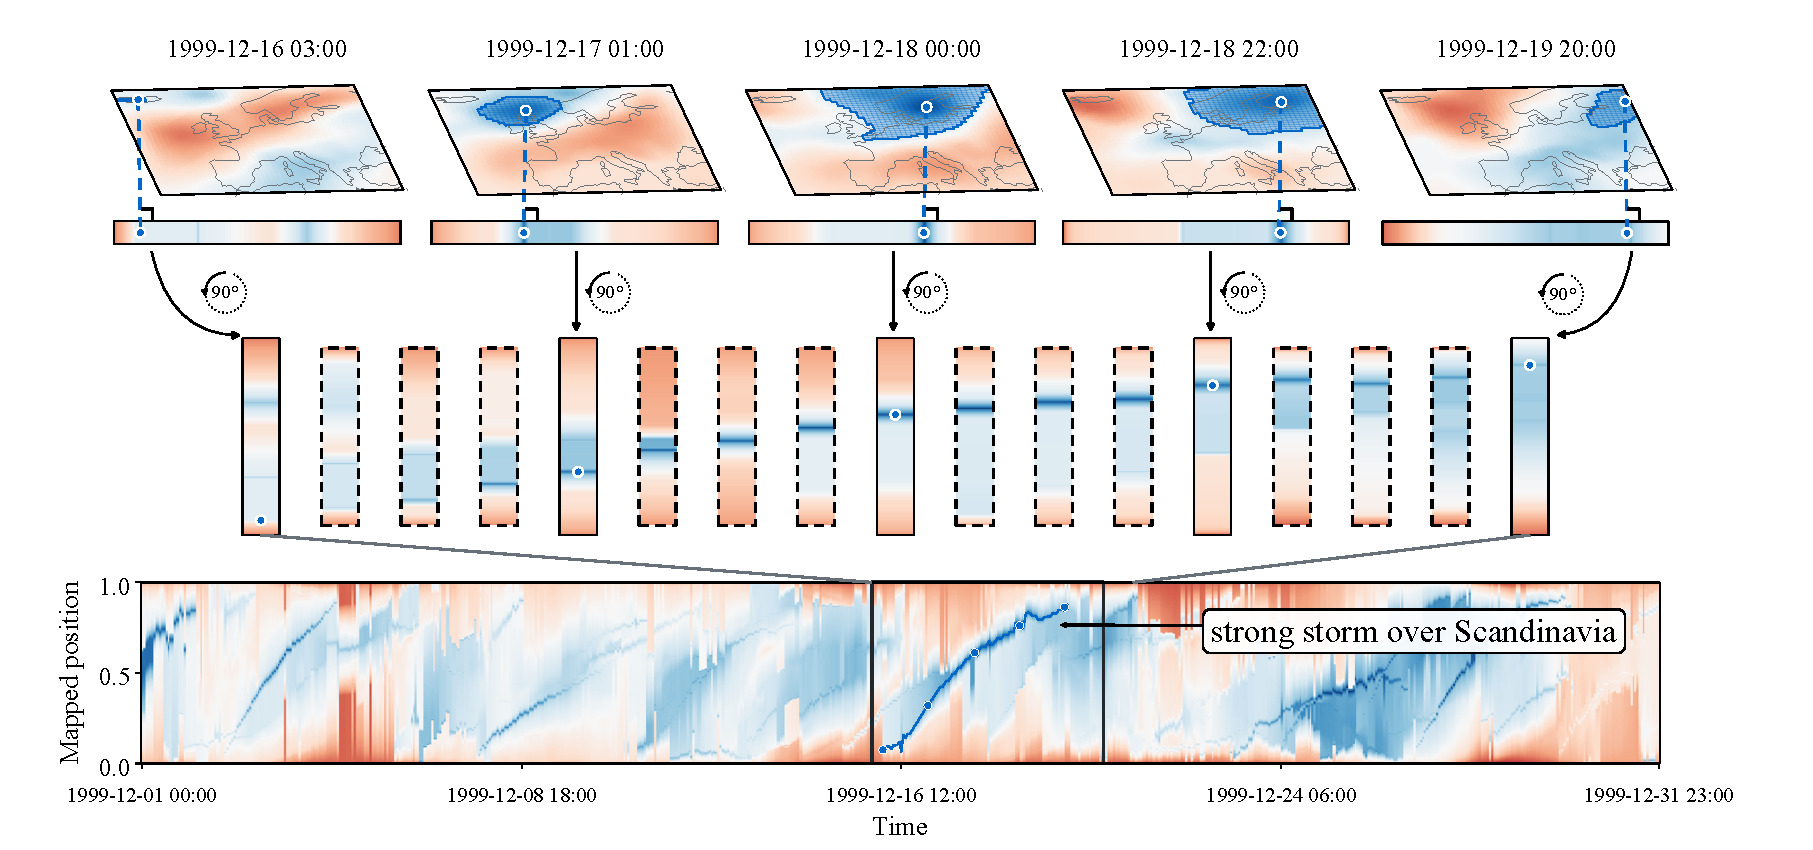
\includegraphics[width=\linewidth]{../figures/anchor_storms_overview.pdf}
\caption{Storms 定性档案（$\varepsilon=5\%$；预处理与表~\ref{tab:quantitative-final} 不同）。空间快照和剖面标出同一个匹配极值；蓝色轮廓为叶弧支撑。旋转后的剖面和虚线框的中间采样帧把它连到完整 744 帧地图中的轨迹。}
\label{fig:storms_overview}
\end{figure}

\section{引言}
一位追踪海上风暴或区域火情的分析者，读时序概览时同时关心三件事：有哪些特征、它们如何嵌套；它们在哪里；它们如何移动。动画保留每一时刻的空间视图，但难以比较相隔较远的时刻；静态概览把一条显示轴给时间，把空间压缩到另一条轴上~\cite{Tversky:2002:Animation,Robertson:2008:Animation,Bach:2017:STC}。第二条轴代表什么，决定了概览能回答上面哪些问题。图~\ref{fig:storms_overview} 把一个特征的空间支撑与这样一张地图联系起来。

合并树图很好地回答了第一个问题。时序合并树图（TMTM）把每一帧的合并树画成一条一维标量剖面，并沿时间对齐这些剖面，极小值表示极值，它们之间的屏障表示合并层级~\cite{Koepp:2023:TMTM}。时空合并树图（ST-MTM）在布局中加入了相对空间距离和时间位置约束~\cite{STMTM:2026}。两者都没有让显示轴具有固定的空间含义：TMTM 按树和时间对齐来排列叶子，而成对距离只固定相对位置，不固定原点或方向。因此特征的位置不能读作它的经度或它沿某个流向的距离，向东移动的特征在图上也不一定移动。Hovm\"oller 图走另一个极端：它保留一个物理坐标，对其余坐标求平均，于是相邻的极值混在一起，层次也消失了~\cite{Hovmoller:1949}。

锚定这条轴，就是把每个极值投影到一个方向上，并把它放在投影位置附近。合并树会阻碍这一点。精确的剖面让每棵子树占据一个连续块，但兄弟子树的投影可能交错。在图~\ref{fig:projection_conflict} 中，四个极小值的投影顺序为 $A,C,D,B$，$C,D$ 子树把 $A$ 和 $B$ 隔开，因此要么有特征离开参考位置，要么有合并层级必须改变；有限的特征宽度还会带来装箱约束。一条空间轴是否值得，取决于层次迫使多少位移，以及用多少合并误差能把位置换回来。

我们回答这两个问题。三个下界给出精确拓扑、有限特征宽度和有界合并误差在每一个可接受布局上迫使的位移；它们只依赖于树、参考和宽度，与求解器无关。AnchorMTM（\emph{Spatially Anchored Merge Tree Maps}，空间锚定合并树图）构造一张接近这些下界的地图：它由匹配极值的运动估计一个参考方向，或采用分析者给定的方向；在合并误差预算 $\varepsilon$ 之内搜索叶序；设置最优合并屏障；用带上限的二次规划放置锚点；并在共同的时间轴上重建标量剖面。精确模式（$\varepsilon=0$）保持合并树；预算模式（$\varepsilon>0$）以声明的合并层级误差换取位置。

我们的主要贡献如下：
\begin{itemize}
\item 把空间锚定合并树图表述为带固定参考和合并层级允许量的层次约束区间布局，并给出精确拓扑、有限宽度和有界合并误差在任何此类布局上迫使的位移的三个下界（第~\ref{sec:bounds} 节）；
\item AnchorMTM：一个只有一个主要控制量 $\varepsilon$ 的构造方法，由运动导出的参考、拓扑预算叶序、最优合并屏障和带上限的时空锚点放置组成（第~\ref{sec:reference} 和~\ref{sec:construction} 节）；
\item 实验评估：下界在受控树上被达到，在 614 个真实平面帧中有 606 帧被所选叶序达到；在 ST-MTM 基准的四个平面序列和两个体数据流场上，AnchorMTM 把特征放得比 TMTM 和 ST-MTM 离参考位置近得多，并且都在声明的合并预算之内（第~\ref{sec:experiments} 节）。
\end{itemize}

\section{相关工作}\label{sec:related}
\subsection{带空间参考的时序可视化}
静态时序显示同时展示相隔较远的观测，动画则保留每一时刻的空间视图；哪种更有用取决于分析任务~\cite{Tversky:2002:Animation,Robertson:2008:Animation}。广义时空立方体描述了联系这些视图的变换~\cite{Bach:2017:STC}。在压缩的时序概览中，空间坐标决定了哪些位置和运动关系可以直接解读。

Hovm\"oller 图保留一个选定的物理坐标并概括其余维度~\cite{Hovmoller:1949}。地理排序和空间填充曲线则遍历整个区域~\cite{Guo:2006:SpatialOrder,Dafner:2000:CSFC}。Dynamic Volume Lines 和数据驱动曲线把空间遍历推广到体数据比较和考虑标量的排序~\cite{Weissenboeck:2019:DVL,Zhou:2021:DSF}。遍历可以保留空间邻域，但它的一维坐标一般不同于固定方向上的投影，而且单靠遍历的相邻关系不能保证合并层次。

一维投影可以组织时空现象~\cite{Franke:2021:1DP}，MotionRugs 展示运动个体的群体行为~\cite{Buchmueller:2019:MR}。更一般地，嵌入要在原始域中的关系与显示组织之间取舍~\cite{Nonato:2019:MP}。相对远近并不能确定绝对坐标。AnchorMTM 为拓扑特征指定固定的投影目标，并量化它们在层次和区间约束下的位移，把空间参考与时序拓扑概览结合起来。

\subsection{基于拓扑的时序地图与几何感知布局}
基于拓扑的可视化通过连通性组织标量结构~\cite{Heine:2016:Survey}。地形景观及其剖面用地形或一维标量表示来表达层次~\cite{Weber:2007:TL,Oesterling:2013:TLP}，并有保持几何和时间连贯的扩展~\cite{Beketayev:2012:GPTL,Herick:2020:TCTL}。这些表示在紧凑的视图中联系标量值与特征关系。

TMTM 在静态合并树图中强调完整的拓扑特征和时间对齐~\cite{Koepp:2023:TMTM}。ST-MTM 加入了相对空间几何和时间位置约束~\cite{STMTM:2026}。这些设计让空间关系和连贯性在地图中发挥作用，但显示坐标仍可以偏离固定的物理方向。AnchorMTM 由极值运动估计一个共同方向，或采用给定的物理方向，并把这个参考与拓扑预算布局和可证明的位置界结合起来。它沿用了已有的剖面和标量填充方法。

层次约束下的叶序传统上最小化相邻元素的差异~\cite{BarJoseph:2001:OLO}；按目标顺序重排的研究讨论了与树相容的排列~\cite{Bulteau:2022:RT}。带分离约束的布局控制几何重叠和位移~\cite{Dwyer:2006:IPSEP,Li:2019:SOI}。AnchorMTM 把这些布局问题与固定的空间目标结合起来。它的精确拓扑点模型叶序界有闭式解，而有限宽度下的候选叶序仍是启发式的。

合并树比较依赖于所用的描述子和对应关系~\cite{Yan:2021:Survey}。带标签的余表型/交错比较支持在固定身份下统计合并层级~\cite{Munch:2019:LINF,Gasparovic:2024:IID}，有序合并树把标量曲线与单调交错距离联系起来~\cite{Beurskens:2025:OMT}。我们用固定标签衡量显示出的合并误差。最优屏障子问题与极小极大超度量拟合有关~\cite{Farach:1995:RM}，额外的限制是所有显示出的合并都由同一个线性顺序决定。

\begin{figure}[t]
\centering
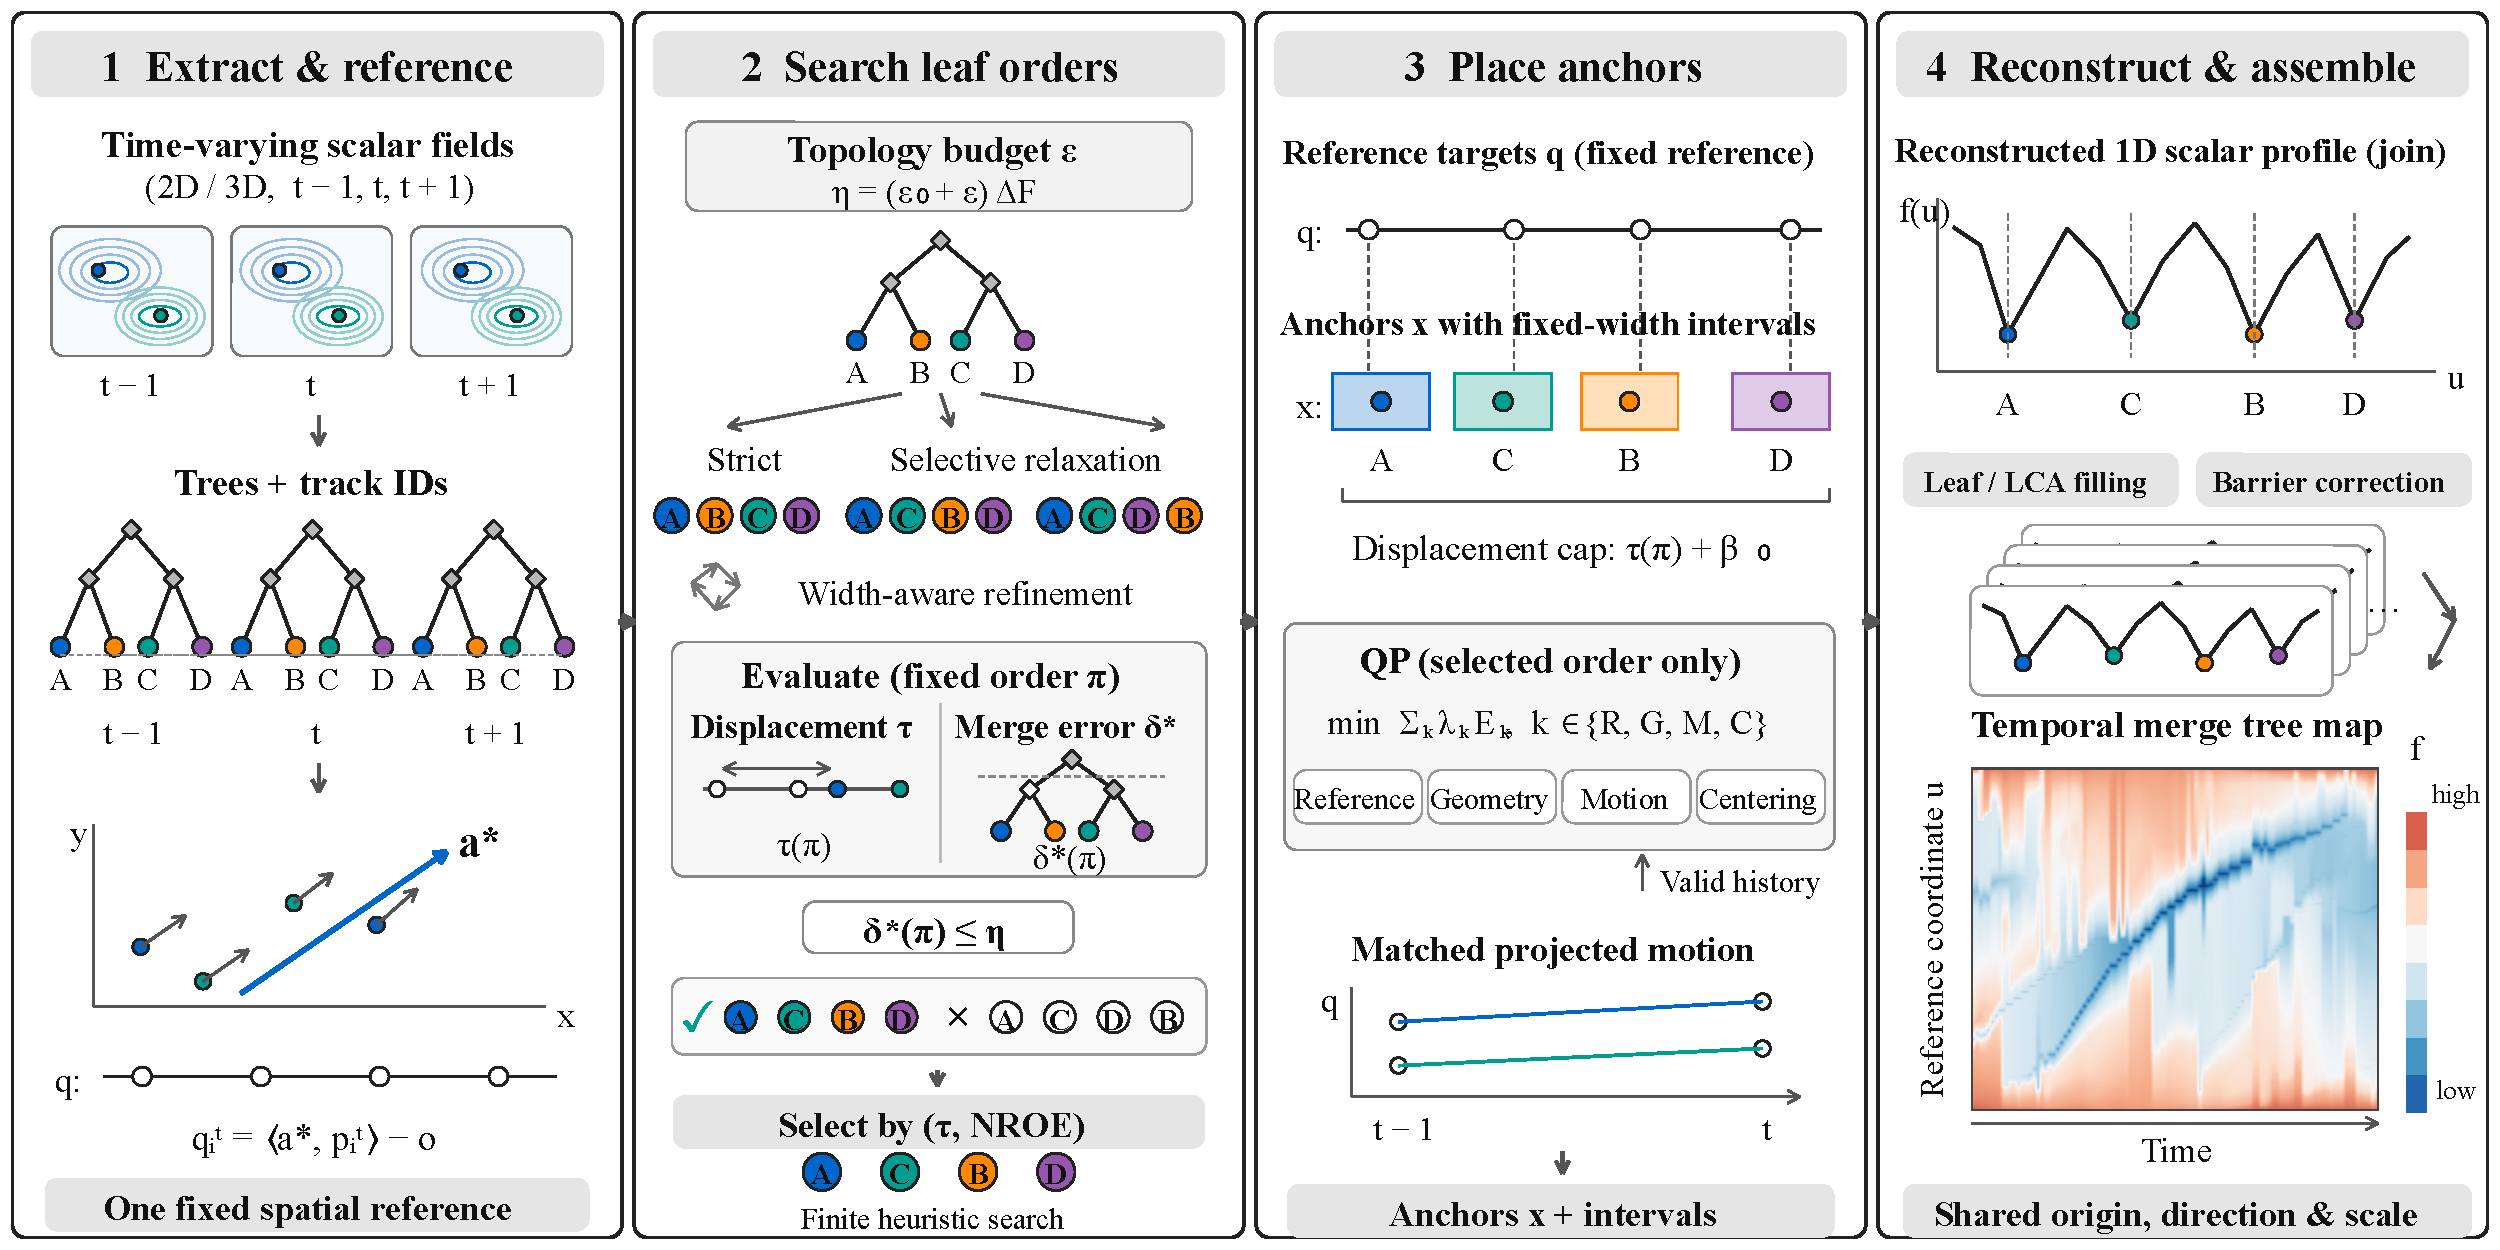
\includegraphics[width=\textwidth]{../figures/anchor_framework.pdf}
\caption{AnchorMTM 的构造流程。(1) 提取增广合并树，匹配叶支撑，再由匹配极值的运动估计一个固定的空间参考。(2) 细化候选叶序，保留满足合并误差允许量的叶序，按固定叶序位移和 NROE 选择。(3) 在互不重叠的区间内、在位移上限下优化锚点，使用有效的匹配历史。(4) 用屏障修正重建标量剖面，组装成时序地图。示意图仅为示意；地图是已有的 Storms 定性结果（$\varepsilon=10\%$）。叶序搜索是启发式的，连续可行性和渲染误差分别检查。}
\label{fig:framework}
\end{figure}

\section{背景}\label{sec:background}
\subsection{增广合并树与特征支撑}
对采样的二维或三维场 $f_t:D\to\mathbb{R}$，合并树 $T_t$ 记录下水平集的连通性：随着阈值升高，极小值产生连通分量，鞍点把它们合并。对场取负即得分裂树约定。临界点是超节点，由超弧相连；增广把正则顶点关联到这些弧上~\cite{Koepp:2023:TMTM,STMTM:2026,Tierny:2018:TTK}。提取和简化在布局之前完成。

一个叶子代表位于空间位置 $p_i^t$ 的一个极值。它的特征支撑 $S_i^t$ 由该极值和其所在叶弧上的正则采样点组成，不含父临界点。它不是整个连通分量，也不是该弧以上的整棵子树。为了做跨帧重叠，这些支撑是稳定的空间采样编号集合：同一个编号在各帧中必须表示同一个空间采样点。固定网格输入通过一致的采样编号保持这一身份。内部弧保留其余正则采样点用于标量填充。记 $\mathcal{D}_t(v)$ 为节点 $v$ 的后代叶标签集合，$h_t(v)$ 为其标量层级。最低公共祖先决定合并高度矩阵：
\begin{equation}\label{eq:merge}
 V_{ij}^t=h_t(\lca(i,j)),\quad i\ne j;\qquad
 V_{ii}^t=f_t(p_i^t).
\end{equation}
同一层级的合并事件构成一个多叉节点；任意的二叉细化不增加严格约束。以下所有保证都针对给定的（可能已简化的）树。

\subsection{一维合并树剖面}
一维合并树剖面在选定的叶序下，把极值画在锚点上。叶弧上的正则顶点提供叶区间内的标量上下文；内部弧和通向最低公共祖先的路径填充中间的间隙~\cite{Koepp:2023:TMTM,STMTM:2026}。在合并约定下，极值成为剖面的极小值，两个锚点之间剖面的最大值就是它们显示出的合并层级。精确保持要求每棵严格子树占据一个连续的叶块。把这些剖面沿时间排列，就得到一张静态时序地图。这一剖面模型是下面空间锚定表述的基础。

\section{AnchorMTM}\label{sec:method}
图~\ref{fig:framework} 概括了构造流程。AnchorMTM 把一个共同的空间参考与显示出的叶锚点联系起来。我们先构造参考并表述布局问题，再描述构造方法，最后用可证明的界解释不可避免的位置代价。分析采用合并约定；分裂树的标量符号在重建后恢复。

\subsection{空间参考与问题表述}\label{sec:reference}
\paragraph{跨帧叶对应。}
我们用叶弧支撑 $S_i^t$ 追踪合并树的叶极值 $p_i^t$。在共同的固定网格上，基于重叠的预处理~\cite{STMTM:2026} 统计共同的空间采样点：
\begin{equation}\label{eq:overlap}
 O_{ij}^t=|S_i^t\cap S_j^{t+1}|.
\end{equation}
匈牙利算法在一对一配对中最大化交集总数，并舍弃重叠为零的配对。分配得到的连接定义下面描述的身份状态。

\emph{延续}继承一个轨迹编号；\emph{出生/消亡}开始一个未匹配的当前身份，或结束一个未匹配的上一条轨迹。对\emph{非双射对应}，包括可能的一对多、多对一和含糊关系，只保留分配到的一对一连接。这些身份状态既不识别物理上的分裂/合并事件，也不构成分支谱系。对当前叶 $i$，$\mu_t(i)$ 表示它的有效前驱。布局接收与叶行对齐的预计算轨迹；上游的支撑和置信度约定见补充材料。

这些对应在任何拓扑预算扫描之前计算，为空间锚定提供运动样本；空间锚定区分参考目标 $q_i^t$ 与显示锚点 $x_i^t$。只有有效的相邻帧匹配贡献位移；匹配失败或轨迹中断的那一步不贡献样本。默认情况下，由所有匹配的相邻帧极值位移离线估计一个单位方向 $a^*\in\mathbb{R}^d$，$d\in\{2,3\}$：
\begin{equation}\label{eq:autodirection}
\begin{aligned}
 \Delta p_i^t&=p_i^t-p_{\mu_t(i)}^{t-1},\\
 S&=\sum_{t,i\;\mathrm{matched}}\Delta p_i^t(\Delta p_i^t)^\top,\\
 a^*&\in\arg\max_{\|a\|=1}a^\top Sa.
\end{aligned}
\end{equation}
主特征向量最大化投影运动的平方和，不考虑特征数量或拓扑相容性。二维和三维用同一个计算，整个序列只算一次。它的符号取为使带符号的投影运动总和非负；若带符号运动接近零，则使绝对值最大的分量为正。若运动能量可以忽略，则取区域最长的坐标轴（并列时取第一个）。主特征值重复时最大化方向不唯一，报告的特征值间隙反映这种不确定性。给定的物理方向可以替代 $a^*$，布局不变。重叠匹配可能漏掉快速移动的特征，或支撑变化、重叠较弱的特征，从而影响位移样本和估计的方向。

\begin{figure}[t]
\centering
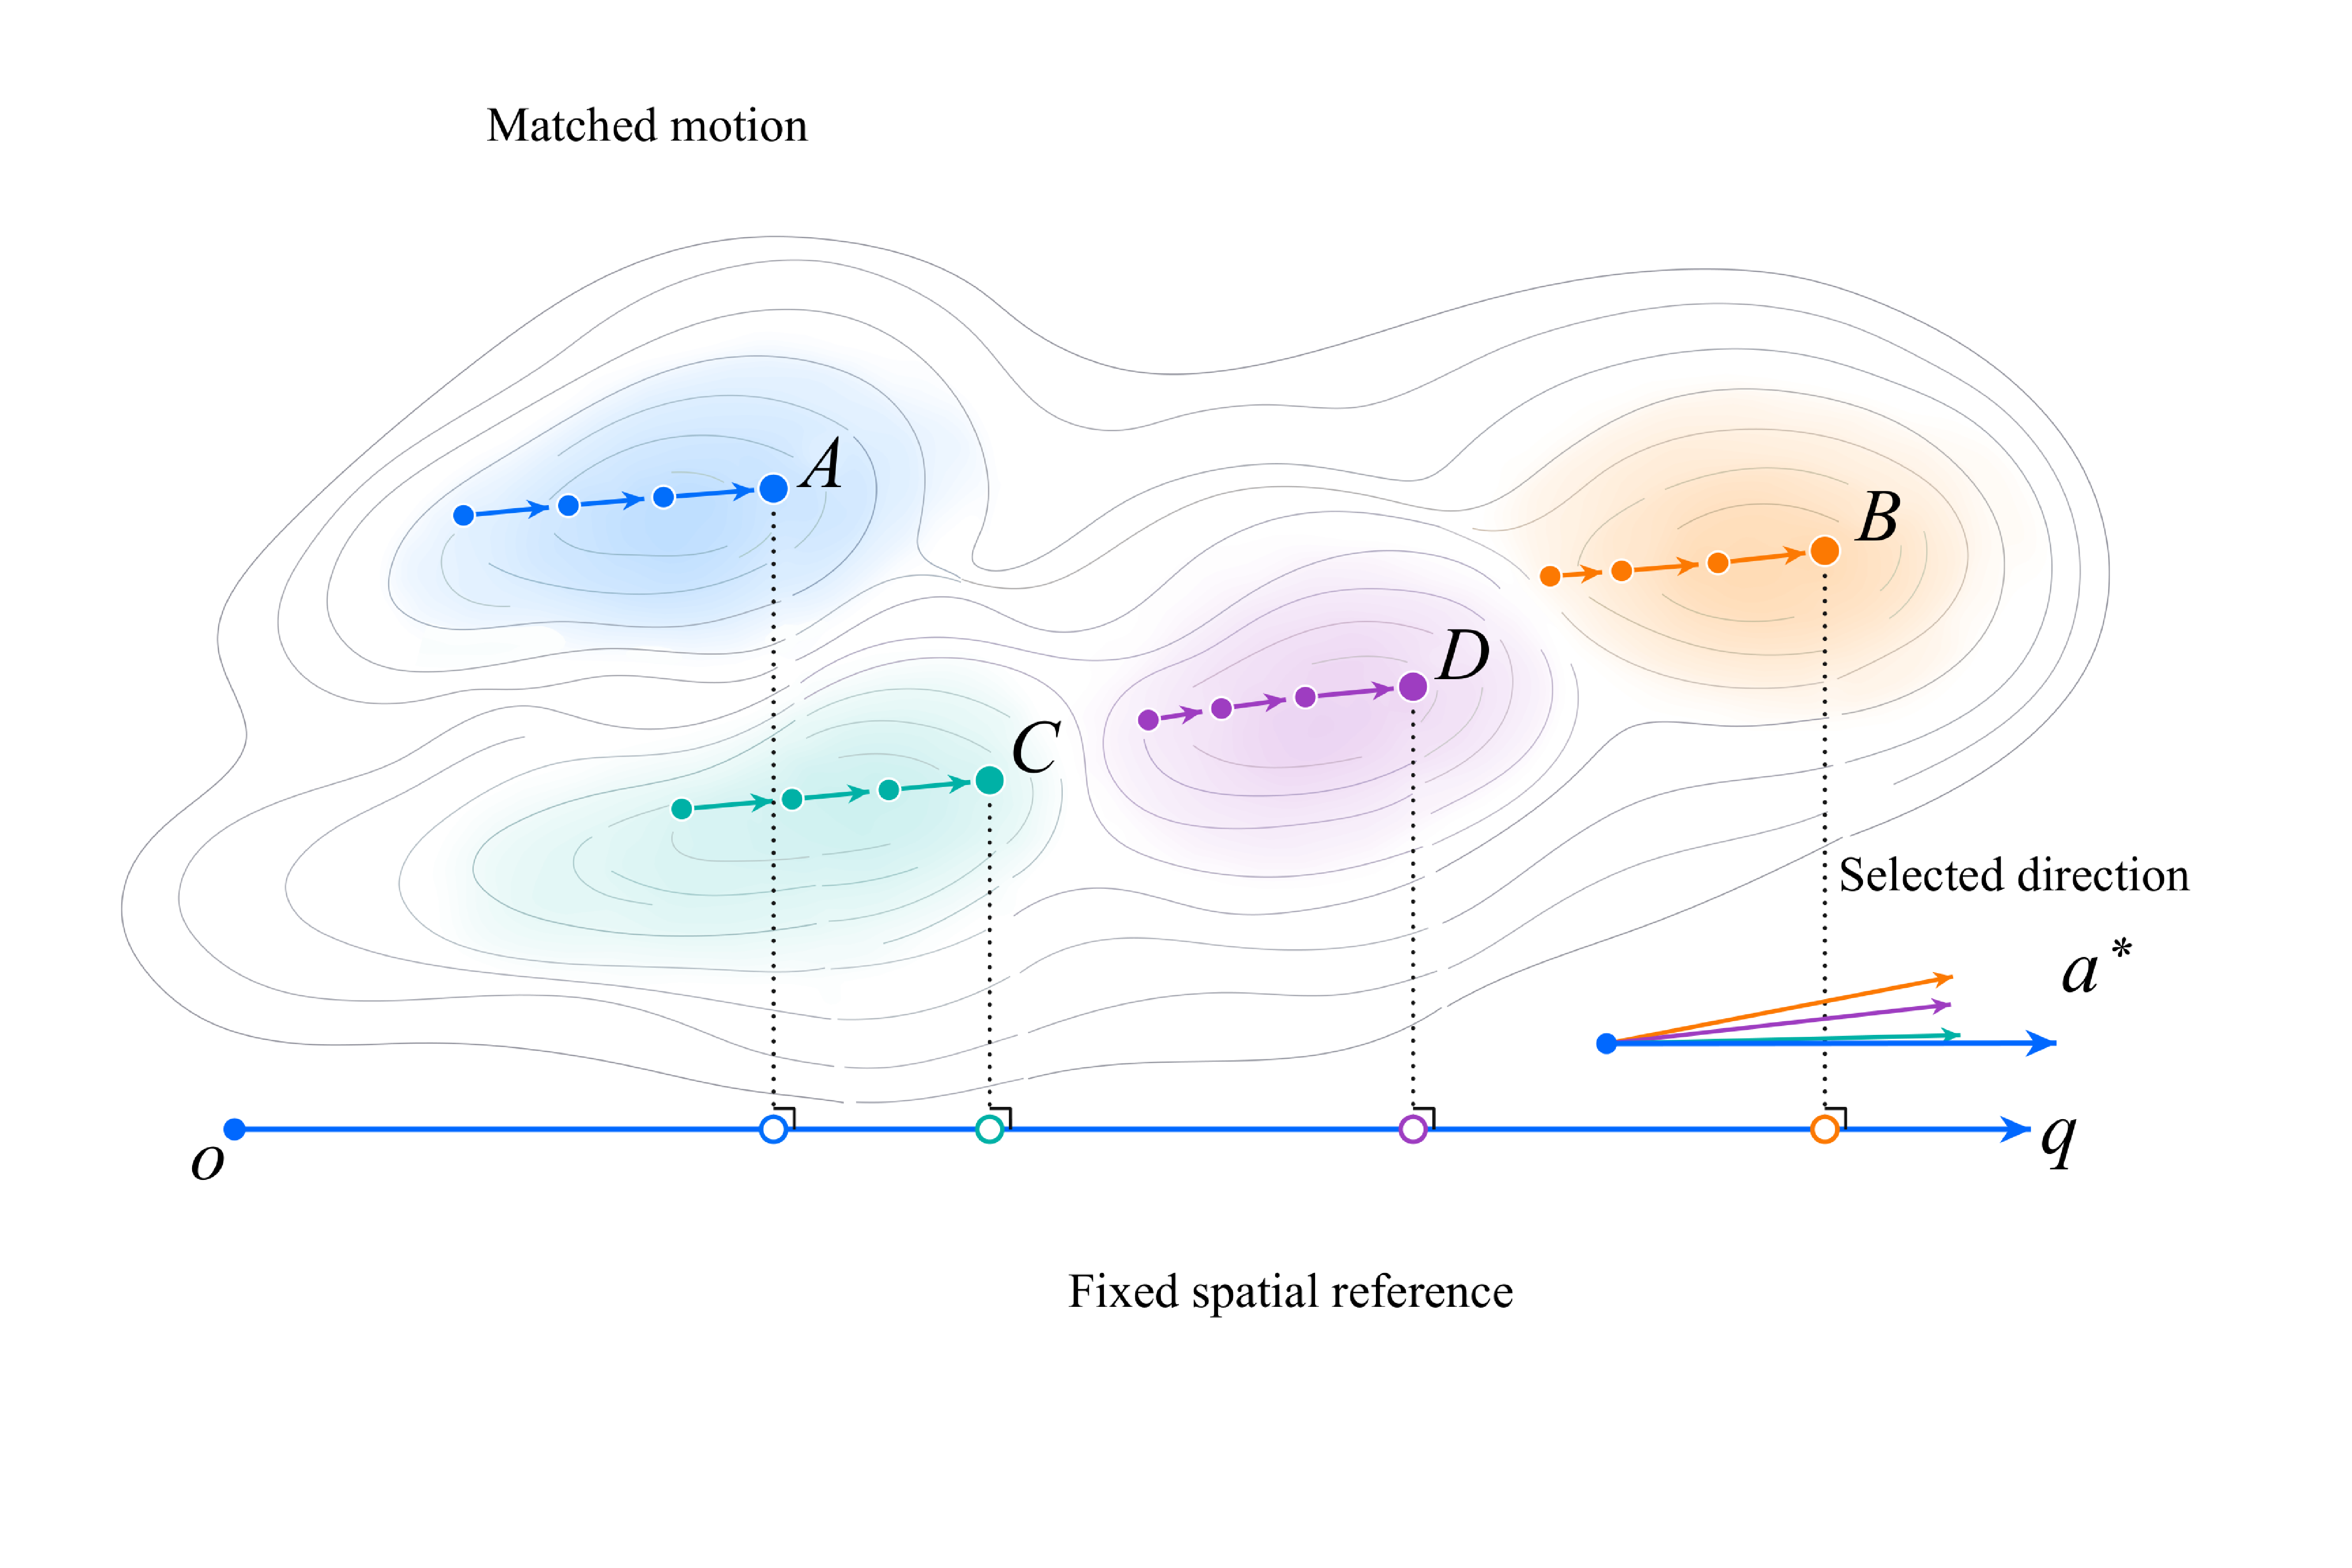
\includegraphics[width=0.6\textwidth]{../figures/anchor_direction_open.pdf}
\caption{由运动导出的空间参考。匹配极值的位移为整个序列确定一个方向 $a^*$；极值从共同原点 $o$ 投影到与之平行的参考轴 $q$ 上。轨迹、等值线和投影位置为示意。}
\label{fig:direction-open}
\end{figure}
图~\ref{fig:direction-open} 示意了这个共同参考。对选定的方向，区域包围盒各角点投影的最小值和跨度确定共同原点 $o$ 和长度 $L>0$。参考为
\begin{equation}\label{eq:reference}
 q_i^t=\langle a^*,p_i^t\rangle-o\in[0,L].
\end{equation}
对同一个预处理后的序列，方向、原点和尺度在所有帧和所有预算下都固定。不同的极值可以有相同的投影坐标，同时保留各自的身份。锚定是在约束下最小化偏离，而不要求 $x_i^t=q_i^t$。

相对几何使用叶支撑质心之间的距离 $d_{ij}^t$。它与极值参考不同，因为支撑变化会移动质心，而极值可能不动。自动参考的适配器显式提供极值；底层求解器也接受预先计算的参考，否则默认使用质心投影。宽度 $W_i^t=s\,m_i^t$ 用固定尺度 $s$ 由正的支撑测度换算，不做逐帧归一化。

图~\ref{fig:projection_conflict} 对比了空间目标顺序与和树相容的顺序。在这个四极小值的例子中，投影顺序 $A,C,D,B$ 让 $C,D$ 子树把 $A$ 和 $B$ 隔开，违反了 $\{A,B\}$ 必须连续的要求；因此精确拓扑不能在不产生位移的情况下实现全部四个目标。

在对应和参考固定之后，一帧由叶序、极值锚点和标量剖面组成：
\begin{equation}\label{eq:mapframe}
 M_t=(\pi_t,x_t,\psi_t),\qquad\psi_t:[0,L]\to\mathbb{R}.
\end{equation}
我们希望位置和运动与参考一致，同时近似相对几何并控制显示出的拓扑。区间布局集合 $\mathcal{L}(\pi)$ 要求以 $z_i$ 为中心、宽度为 $W_i$ 的区间位于画布内，互不相交且间隔至少为 $g\ge0$，并包含满足 $|x_i-z_i|\le\rho W_i/2$（$0\le\rho\le1$）的锚点。总宽度和间隔放不下时报告失败，而不是缩放。

实际位移为 $|x_i-q_i|$，报告时除以 $L$。为了区分叶序冲突与有限宽度放置，定义
\begin{equation}\label{eq:nroe}
 \nroe(\pi)=\frac{1}{2L}\max_{j\le k}
                      [q_{\pi(j)}-q_{\pi(k)}]^+.
\end{equation}
它是单调非减的点放置的最小最坏位移除以 $L$，不考虑宽度。对有限区间，固定叶序的精确代价为
\begin{equation}\label{eq:tau}
 \tau(\pi)=\min_{(x,z)\in\mathcal{L}(\pi)}\|x-q\|_\infty.
\end{equation}
只要布局集合非空，最小值就能取到。它由固定叶序的装箱约束精确求出，等价于一个极小极大线性规划。

对不同的标签，记 $V_{ij}^{\psi}$ 为它们锚点之间剖面的最大值，并令 $V_{ii}^{\psi}=\psi(x_i)$。我们要求
\begin{equation}\label{eq:dtop}
\begin{aligned}
 \dtop(\psi_t,T_t)&=\max_{i,j}|V_{ij}^{\psi_t}-V_{ij}^t|\le\eta,\\
 \eta&=(\varepsilon_0+\varepsilon)\Delta_F.
\end{aligned}
\end{equation}
其中 $\Delta_F>0$ 是整个序列的标量范围，$\varepsilon_0$ 是固定的数值允许量，$\varepsilon\ge0$ 是唯一的主要用户控制量。实现中默认 $\varepsilon_0=10^{-7}$。NMLE 报告实际达到的归一化误差 $\dtop/\Delta_F$。精确拓扑指在给定的树上标签误差为零。非零的并列允许量计入 $\eta$。

其余所有设置都属于固定配置 $\Theta_0$：位置松弛 $\beta_0$、四个目标权重、宽度尺度、间隔、锚点松弛和输出分辨率。对一个预处理后的序列，默认接口为 $M_t^\varepsilon=\operatorname{AnchorMTM}(T_t,q_t,W_t,V_t,\mu_t;\varepsilon,\Theta_0)$。高级设置可以一次性给定，但在预算扫描中只有 $\varepsilon$ 变化。补充材料给出固定的尺度规则和实现容差。

对于固定标签覆盖所有叶、诱导矩阵包含对角线的规范余表型合并树表示，$\dtop$ 等于未归一化的带标签交错距离~\cite{Munch:2019:LINF,Gasparovic:2024:IID}。在这些条件下 $d_B\le d_I\le\dtop$~\cite{Morozov:2013:IDMT}。渲染引入的无标签极值必须先检查，才能把这一解释用于整棵显示出的树。

\begin{figure}[t]
\centering
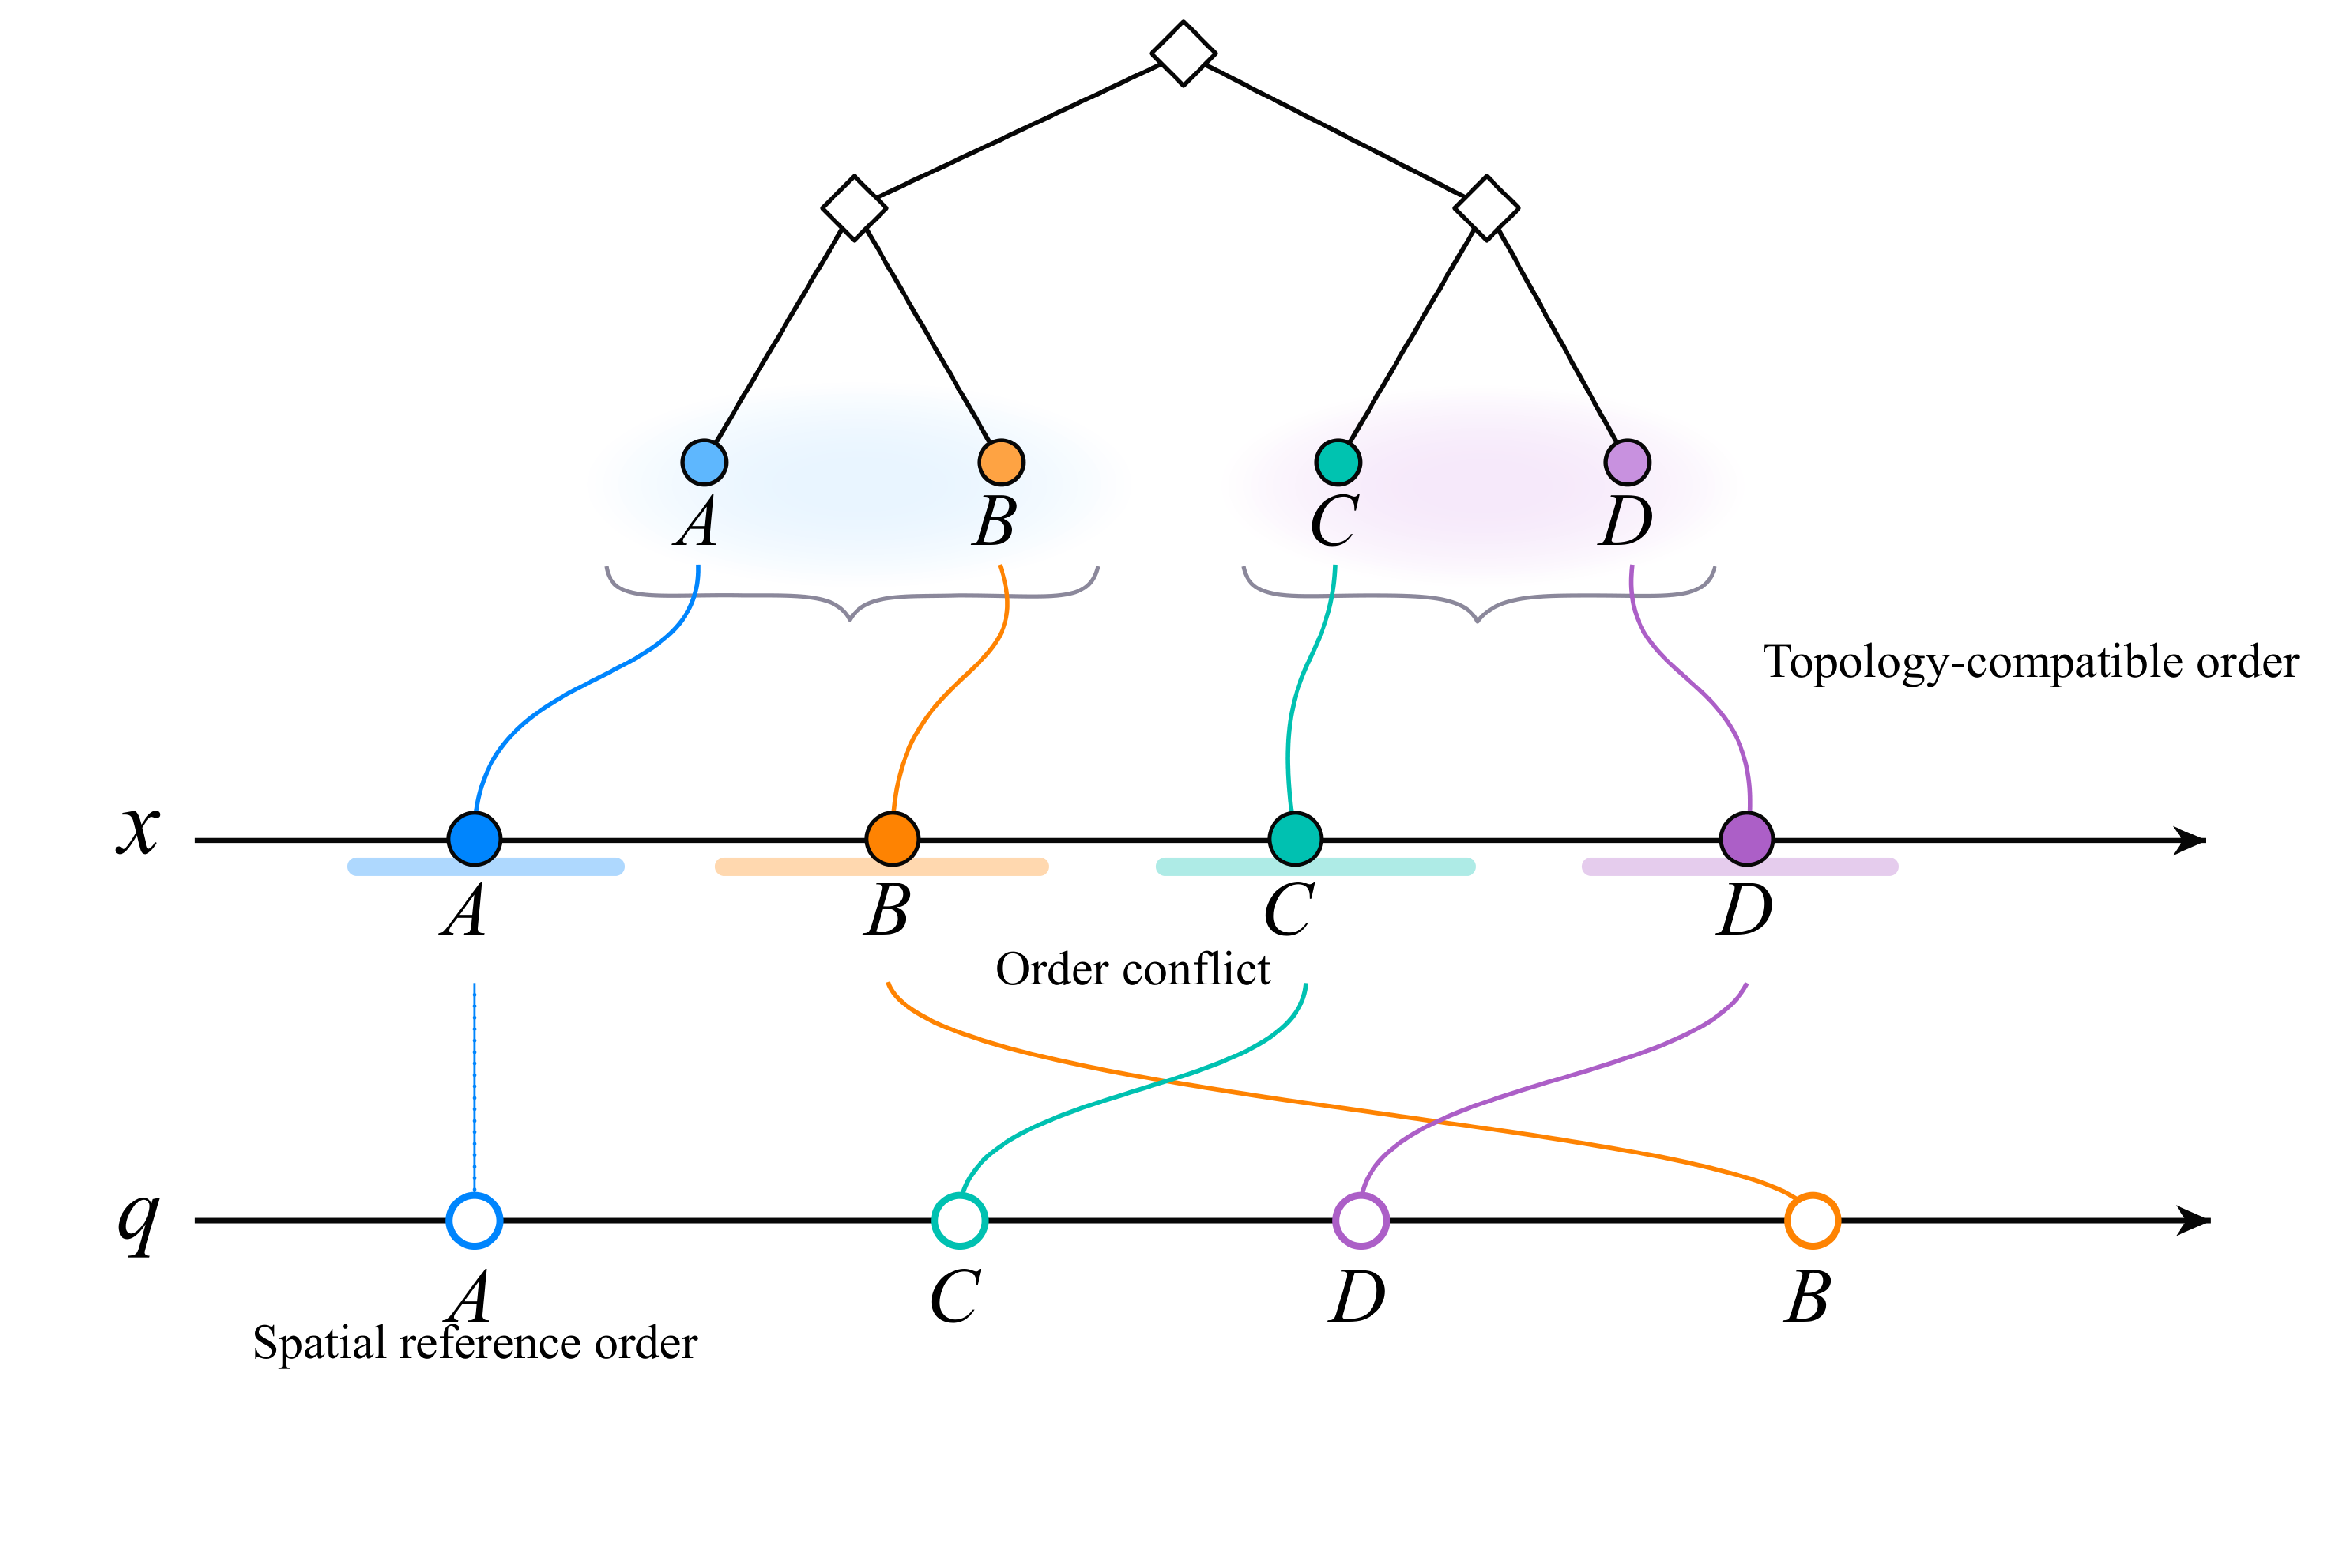
\includegraphics[width=0.7\textwidth]{../figures/anchor_conflict_open.pdf}
\caption{参考与拓扑的冲突。树要求 $A,B$ 和 $C,D$ 各自连续。显示的锚点 $x$ 按相容的顺序排列，而固定的空间目标 $q$ 的顺序是 $A,C,D,B$。彩色连线表示调和两种顺序所需的位移。宽度和位置为示意。}
\label{fig:projection_conflict}
\end{figure}

\subsection{空间锚定布局的构造}\label{sec:construction}
在特征及其参考固定后，构造按字典序目标选择叶序：
\begin{equation}\label{eq:orderobjective}
\begin{aligned}
 \pi_t^\varepsilon&\in\underset{\pi\in\mathcal{C}_t(\varepsilon)}{\arg\min}
                    \bigl(\tau_t(\pi),\nroe_t(\pi)\bigr),\\
 &\hspace{1em}\mathrm{s.t.}\quad\delta_t^*(\pi)\le\eta(\varepsilon).
\end{aligned}
\end{equation}
有限的候选池包含原始的严格拓扑叶序、中点初始化的叶序，以及在阈值展平和选择性展平上做宽度感知细化时访问过的叶序。每个候选都对照同一个源合并矩阵评估。选择时先最小化 $\tau$，再最小化 NROE；这不是对所有排列的全局最优。算法~\ref{alg:construction} 把这一离散选择与固定叶序下的放置分开。

\begin{algorithm}[htbp]
\caption{单控制量 AnchorMTM}\label{alg:construction}
\KwData{二维/三维场序列及网格；$\varepsilon\ge0$；固定配置 $\Theta_0$。}
\KwResult{时序地图 $I^\varepsilon$、误差记录或失败报告。}
提取增广树、叶支撑和极值；匹配支撑并分配轨迹编号\;
估计一个方向和固定参考 $q_t$；该预处理在各预算间复用\;
$\eta\leftarrow(\varepsilon_0+\varepsilon)\Delta_F$\;
\For{按时间顺序的每一帧 $t$}{
 若宽度和间隔超出固定画布，报告并停止\;
 $\mathcal{C}_t\leftarrow\operatorname{GenerateAndRefine}(T_t,q_t,W_t,V_t,\eta)$；保留严格拓扑候选\;
 对候选计算 $\tau(\pi)$、$\nroe(\pi)$ 和 $\delta^*(\pi)$\;
 $\mathcal{F}_t\leftarrow\{\pi\in\mathcal{C}_t:\delta^*(\pi)\le\eta\}$\;
 \lIf{$\mathcal{F}_t=\varnothing$}{报告没有可行候选并停止}
 按 $(\tau,\nroe)$ 从 $\mathcal{F}_t$ 中选出 $\pi_t^\varepsilon$\;
 为 $\pi_t^\varepsilon$ 计算最优合并屏障\;
 只对 $\pi_t^\varepsilon$ 求解四项二次规划，上限为 $\tau(\pi_t^\varepsilon)+\beta_0$，使用有效的匹配历史\;
 用叶/最低公共祖先填充和屏障修正重建剖面\;
 记录候选数、连续与渲染误差、运动和失败；把剖面加入 $I^\varepsilon$\;
}
\KwReturn{$I^\varepsilon$ 和诊断记录}\;
\end{algorithm}

\subsubsection{拓扑预算叶序}
\emph{精确模式}取 $\varepsilon=0$，只保留数值允许量 $\eta=\varepsilon_0\Delta_F$，它只合并相差在 $\varepsilon_0\Delta_F$ 以内的鞍点；严格的精确拓扑是 $\eta=0$。\emph{预算模式}允许 $\varepsilon>0$。两种模式使用相同的区间模型和放置目标。

候选生成包括原树、阈值展平和一个由冲突驱动的选择性展平。这些结构用中点叶序初始化。宽度感知的块插入细化最好的四个初始结构以及原树，同时保留点模型的预算叶序作为候选。每一步移动都要改进由 $\tau$ 和一个装箱残差平方项组成的字典序得分，并且必须通过 $\delta^*(\pi)\le\eta$。访问过的初始叶序和试探叶序都保留在去重后的候选池中，包括严格树的初始化和保留的点模型候选。最终的预算筛选和字典序选择使用精确的固定叶序代价；细化过程不保证对所有排列全局最优。

图~\ref{fig:selective_relaxation} 示意了选择性展平带来的额外叶序自由度。去掉 $A$--$B$ 的兄弟约束后，允许叶序 $A,C,D,B$，同时保留 $C$--$D$ 子树。这一结构上的提议仍需对照原始合并矩阵和规定的误差预算评估。

辅助函数沿用当前的几何和布局参数。比较使用实现中的数值容差。保护机制会报告容量失败或候选集合为空；不会悄悄改变宽度、间隔或画布尺度。原树结构始终保留在细化起点中，它的子块移动在精确模型中保持严格拓扑。它的存在不保证数值放置或栅格重建一定成功；容量、输入和求解器失败仍可能发生。不会从空的候选集合中做选择。无效输入和数值求解失败作为错误报告，与数学上的不可行区分开。第一帧和未匹配的历史不提供时间目标。

\subsubsection{最优合并屏障与拓扑可行性}
对固定的叶序，一对叶子显示出的合并层级是它们之间最大的屏障。对间隙 $k$，令
\[
 C_k=\min_{i\le k<j}V_{\pi(i)\pi(j)},\qquad F_k=\max(V_{\pi(k)\pi(k)},V_{\pi(k+1)\pi(k+1)}).
\]
\begin{proposition}[最优屏障]\label{prop:barriers}
在极值固定的连续非严格模型中，最小的标签合并误差为
\begin{equation}\label{eq:delta}
\begin{split}
 \delta^*(\pi)=\max\bigg\{&0,\max_k(F_k-C_k),\\
 &\frac12\max_{i<j}\left(V_{\pi(i)\pi(j)}-
                         \max_{i\le k<j}C_k\right)\bigg\},
\end{split}
\end{equation}
屏障 $b_k=C_k+\delta^*(\pi)$ 达到这一误差。
\end{proposition}
误差 $\delta$ 要求 $F_k\le b_k\le C_k+\delta$。取最大的可行屏障，当且仅当 $\delta\ge\delta^*$ 时满足每一对的合并下限要求。因此在这一连续模型中，叶序满足合并层级允许量当且仅当 $\delta^*(\pi)\le\eta$。这一固定叶序检验支撑候选搜索，但不使搜索全局最优。严格极值间隙和栅格效应另行检查。

\subsubsection{空间锚定的时空放置}
叶序固定后，核心项是 $E_R$（与固定参考的均方偏差）和 $E_M$（匹配的投影运动的均方误差）。辅助项 $E_G$ 通过有序锚点间距近似支撑质心之间的距离；$E_C$ 约束锚点相对区间中心的偏移。四项及其非负权重都保留：
\begin{equation}\label{eq:qp}
\begin{aligned}
 \min_{x_t,z_t}\quad&\lambda_R E_R+\lambda_G E_G+\lambda_M E_M+\lambda_C E_C\\
 \mathrm{s.t.}\quad&(x_t,z_t)\in\mathcal{L}(\pi_t),\\
 &\|x_t-q_t\|_\infty\le\tau(\pi_t)+\beta_0.
\end{aligned}
\end{equation}
对每个有效匹配，令 $\Delta q_i^t=q_i^t-q_{\mu_t(i)}^{t-1}$，并把上一帧的显示锚点加上这一参考位移作为时间目标：
\begin{equation}\label{eq:temporal_target}
 \hat x_i^t=x_{\mu_t(i)}^{t-1}+(q_i^t-q_{\mu_t(i)}^{t-1}).
\end{equation}
因此 $E_M$ 跟随投影运动，同时倾向于让 $x-q$ 连续。第一帧、新出生和其他未匹配的叶子没有上一帧的运动惩罚。每一项分别对其特征、有序对或有效匹配取平均；当前的自动参考适配器对有效匹配使用单位置信度。补充材料区分了这一默认设置与旧的置信度加权路径。

只有 $\varepsilon$ 改变拓扑允许量 $\eta(\varepsilon)$。固定松弛 $\beta_0\ge0$ 限制排序之后额外的位置偏差。由于 $\tau(\pi_t)$ 可以取到，这个上限总是可行；二次规划只接收选定的叶序，不能换成二次目标更低的其他叶序。上限约束连续位移，几何和时间目标在上限之内选择折中。固定叶序的问题是凸的；逐帧顺序求解并不意味着整个序列的联合最优，也不保证精确保持每一个投影运动。

\subsubsection{剖面重建与输出诊断}
重建沿用合并树图流程中的叶弧采样和最低公共祖先路径填充~\cite{Koepp:2023:TMTM,STMTM:2026}。原始极值保持在锚点上；正则采样点为区间和间隙提供标量上下文。最优屏障修正再把每段锚点之间的内部值截断到 $b_k$，必要时抬高已有的峰。放宽后的叶序需要这一单独的修正；仅靠沿用的最低公共祖先填充不能保证极小极大屏障。

所有帧使用同一个方向、原点、长度和像素换算。各剖面构成最终的时序地图
\begin{equation}\label{eq:map}
 I^\varepsilon(t,u)=\psi_t^\varepsilon(u),\qquad 0\le u\le L.
\end{equation}
不做逐帧重新居中。重采样不会保留每一个源采样点，修正后的内部值也不一定在原始标量范围之内。严格极值间隙和栅格取整会改变实际达到的误差。对整棵树的解释还需要检查标签覆盖。因此记录下来的剖面并不无条件地被 $\delta^*\le\eta$ 证明。记录中区分请求的预算、位置证书、实际的 $\tau$、连续的 $\delta^*$ 以及实际渲染的误差。

\begin{figure}[t]
\centering
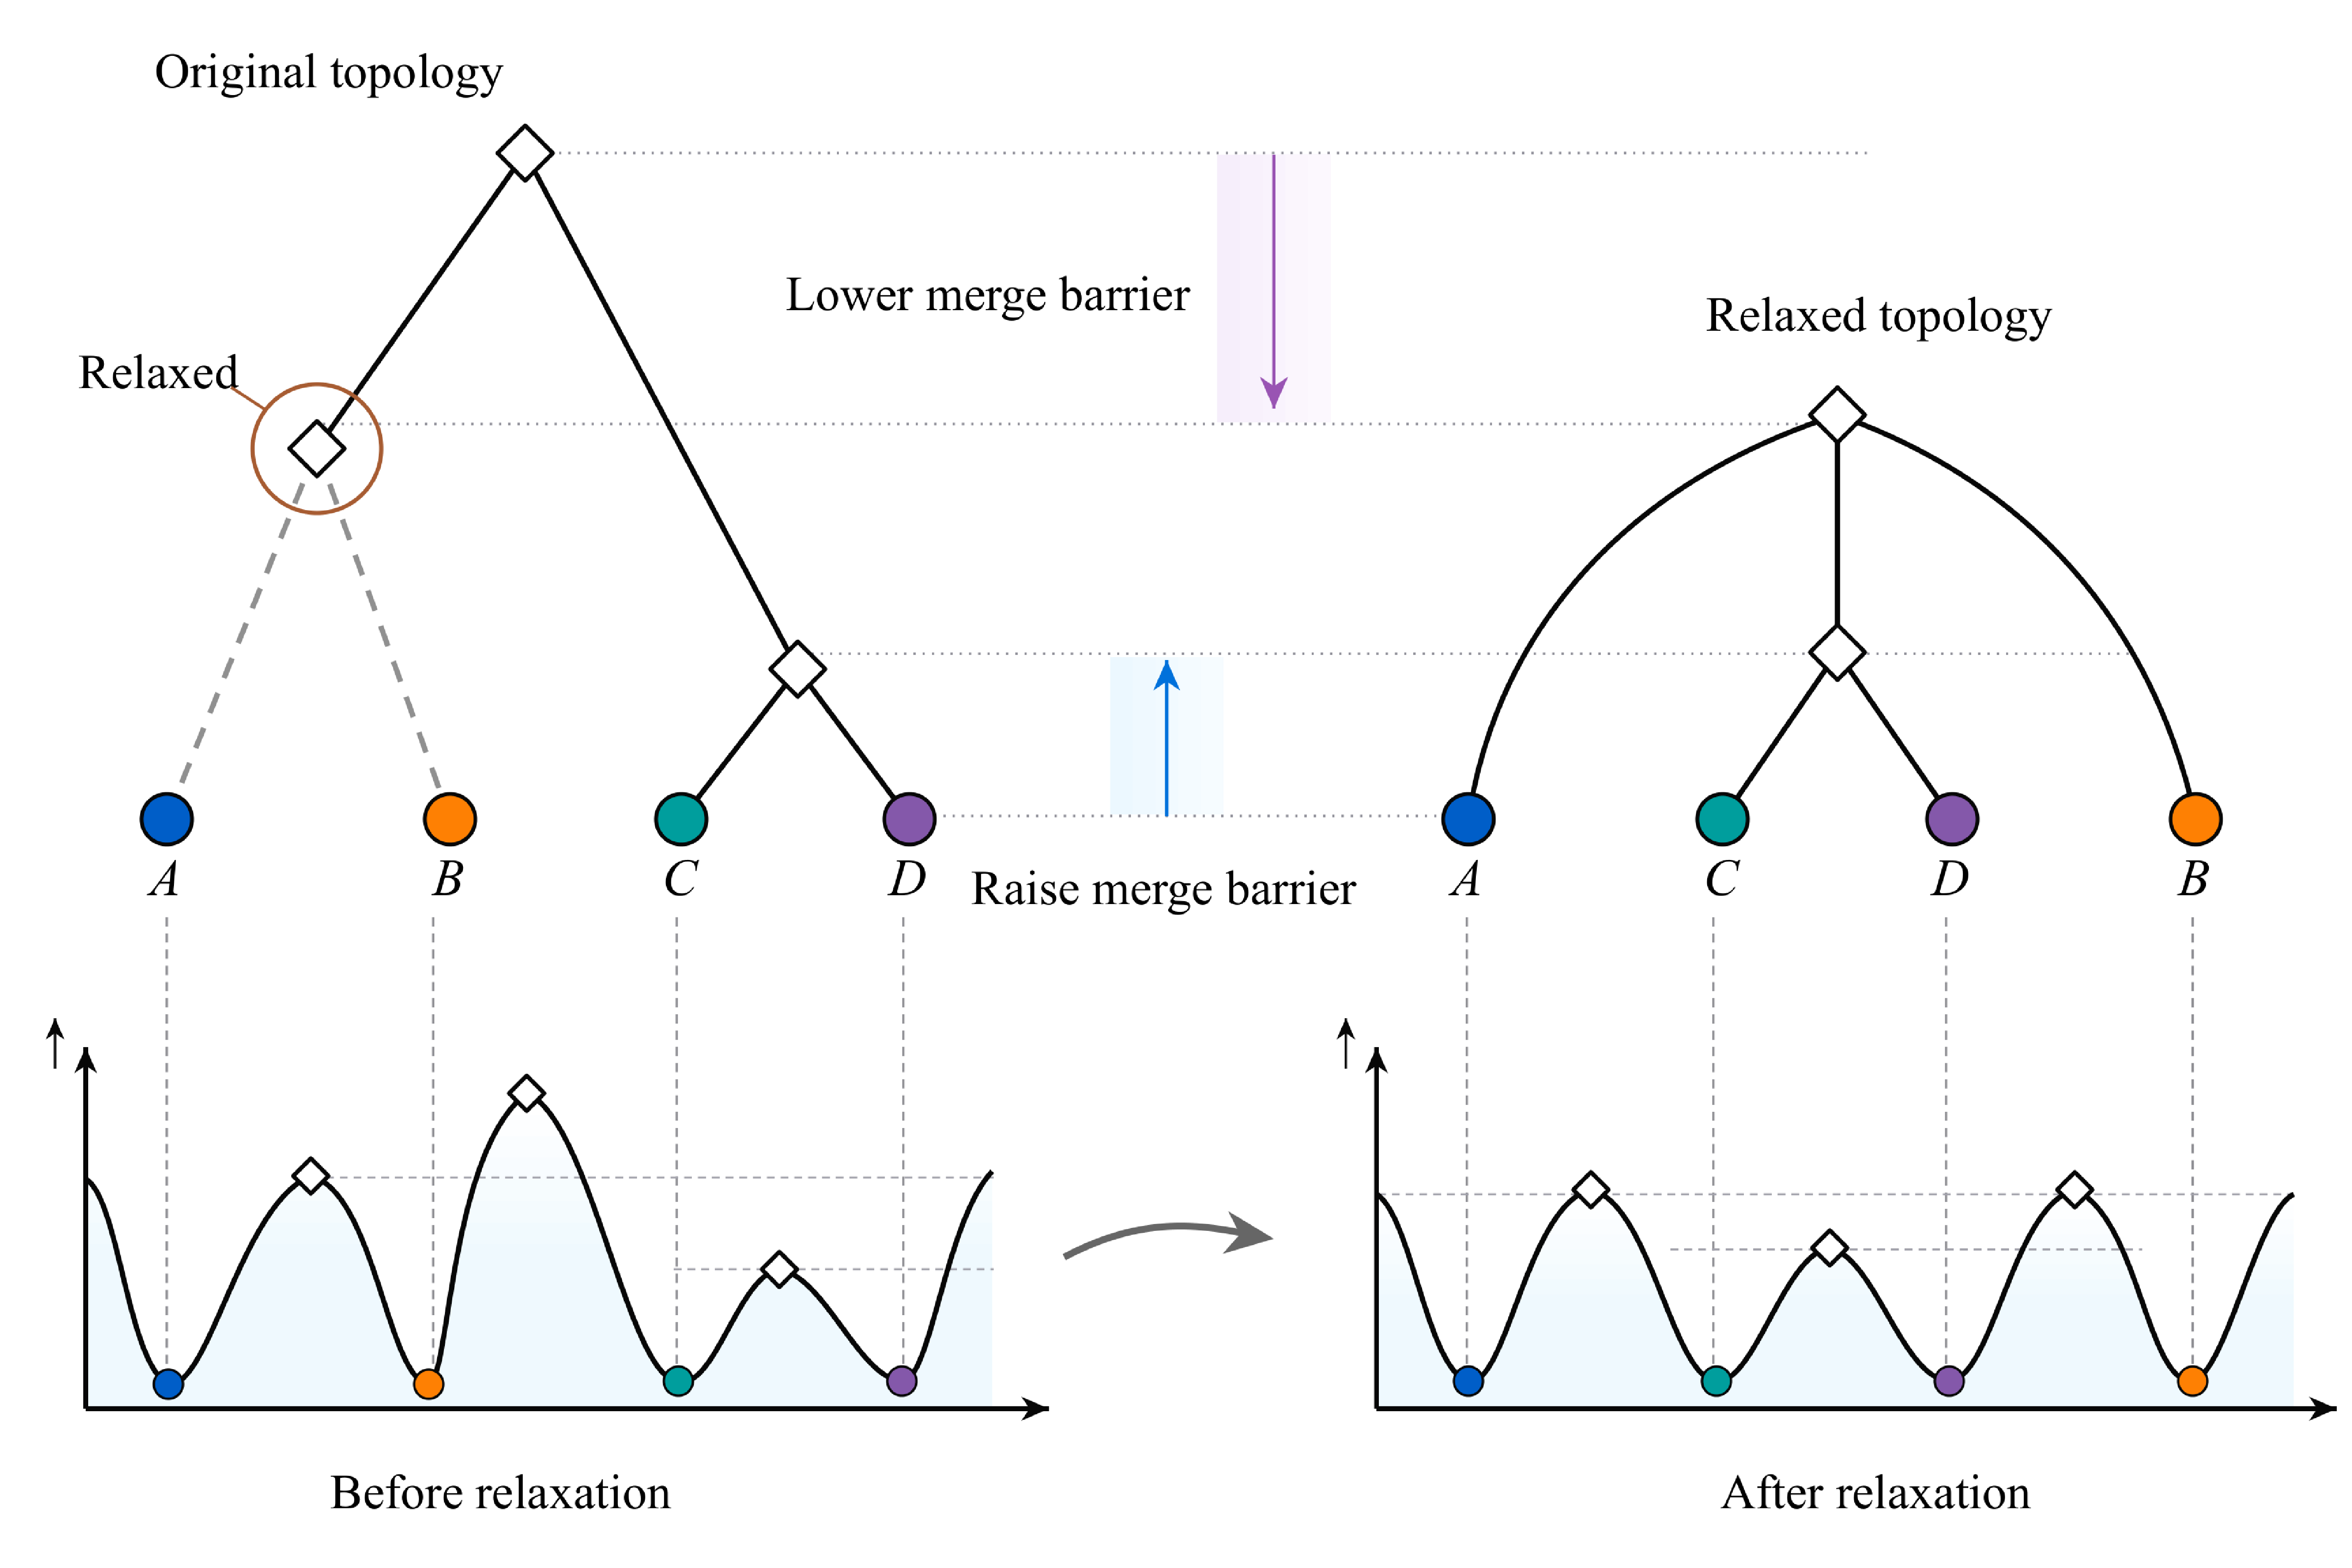
\includegraphics[width=0.7\textwidth]{../figures/anchor_relaxation_open.pdf}
\caption{选择性放宽解除 $A,B$ 的块约束，允许叶序 $A,C,D,B$，同时保留 $C,D$ 分组。附带的剖面示意屏障的变化；源层级的引导线表示层次的变化。高度为示意，候选叶序仍需对照原始合并矩阵评估。}
\label{fig:selective_relaxation}
\end{figure}

\subsection{可证明的位置–拓扑界}\label{sec:bounds}
即使经过优化，构造仍可能留下参考位移。下面的界说明拓扑和有限宽度使哪些位移不可避免：第一个界回答与树相容的点叶序必须偏离多少，第二个界加入区间装箱，第三个界问在合并误差允许量下还剩哪些限制。它们是分析用的基准，不是三个执行阶段，也不是剪枝规则；构造使用精确的固定叶序代价 $\tau$ 和 $\delta^*$。得到的证书与布局算法无关。完整证明和计算定义见补充材料。在一帧之内省略 $t$，记 $[v]^+=\max(v,0)$，并约定空集上的最大值为零。

\subsubsection{精确拓扑的参考叶序界}
对真祖先层级严格递增的约化树，精确拓扑使每棵子树连续。记 $[m_X,M_X]$ 为子树 $X$ 中叶子参考位置的范围。
\begin{theorem}[精确拓扑位置界]\label{thm:order}
每个零误差剖面满足 $\nroe(\pi)\ge\nu^*(T,q)$，其中
\begin{equation}\label{eq:nu}
 \nu^*(T,q)=\frac{1}{2L}\max_v\max_{\substack{X,Y\in\mathrm{ch}(v)\\X\ne Y}}
 [\min(M_X-m_Y,M_Y-m_X)]^+.
\end{equation}
按参考范围中点递归排列子节点，可在 $O(n\log n)$ 时间内达到这一点模型叶序界。
\end{theorem}
\begin{proof}[证明概要]
兄弟块必须选择一个先后方向。两种方向的逆序代价分别为 $[M_X-m_Y]^+/2$ 和 $[M_Y-m_X]^+/2$。中点排序选择较小者；每一对逆序的叶子都在其最低公共祖先处被兄弟块隔开。
\end{proof}
这一结果单独刻画了树和参考带来的叶序限制。中点排序达到点模型叶序的最优；有限区间带来额外的约束，见下文。

\subsubsection{宽度感知位置界}
有限宽度、最小间隔、锚点松弛和画布容量在点叶序障碍之上增加装箱代价。对非空叶集合 $S$，令 $H_i=\rho W_i/2$，$\ell_i=q_i-W_i/2-H_i$，$h_i=q_i+W_i/2+H_i$，$s_i=W_i+g$。定义两个装箱量：
\begin{equation}\label{eq:packing}
\begin{aligned}
 A(S)&=\max_{a\in S}\left(\ell_a+\sum_{\substack{i\in S\\\ell_i\ge\ell_a}}s_i\right),\\
 B(S)&=\max_{b\in S}\left(\sum_{\substack{i\in S\\h_i\le h_b}}s_i-h_b\right).
\end{aligned}
\end{equation}
前者使用参考端点的上集，后者使用下集；排序加前缀和即可计算。对不相交的叶集合 $X,Y$ 和全部叶集合 $\mathcal{F}$，记
\begin{equation}\label{eq:packingcost}
\begin{aligned}
 \omega(X,Y)&=\tfrac12\min\{A(X)+B(Y),A(Y)+B(X)\}-\tfrac g2,\\
 E_\partial&=\max\{0,B(\mathcal{F})-g,A(\mathcal{F})-g-L\}.
\end{aligned}
\end{equation}
其中 $\omega$ 取代价较小的块方向，$E_\partial$ 计入画布两端。令 $\mathcal{P}_0$ 包含所有不同兄弟后代叶集合构成的对。证书为
\begin{equation}\label{eq:bwdef}
 \mathcal{B}_w(T,q,W)=\max\{E_\partial,\max_{(X,Y)\in\mathcal{P}_0}\omega(X,Y)\}.
\end{equation}
它通过式~\eqref{eq:packing}--\eqref{eq:packingcost} 依赖于 $g$、$\rho$ 和 $L$，证书的自变量中省略不写。
\begin{theorem}[宽度感知位置界]\label{thm:width}
对任何可行的精确拓扑区间布局，
\begin{equation}\label{eq:widthbound}
 \|x-q\|_\infty\ge\tau(\pi)\ge\mathcal{B}_w(T,q,W).
\end{equation}
宽度和间隔为零时，$\mathcal{B}_w=L\nu^*(T,q)$。
\end{theorem}
\begin{proof}[证明概要]
选定叶子中第一个和最后一个锚点之间，必须容纳它们的区间和中间的间隔（锚点松弛范围内）。式~\eqref{eq:packing} 中的上集和下集使由此产生的、相对参考间距的不足量最大。精确拓扑要求每一对兄弟选择一个方向；画布两端给出两个单侧代价。
\end{proof}
因此 $\mathcal{B}_w$ 是所有精确拓扑合法区间叶序的下界，不一定能达到；$\tau(\pi)$ 是给定叶序下实际达到的最小值。这些量的单位是坐标单位，而 NROE 和 $\nu^*$ 除以了 $L$。

\subsubsection{有界拓扑位置界}
合并层级允许量可以解除一部分连续块的约束，但仍然限制交错。若叶 $k$ 位于节点 $u$ 的两个后代 $i,j$ 之间，区间包含关系给出 $V_{ik}^{\psi}\le V_{ij}^{\psi}$，从而 $V_{ik}\le h(u)+2\eta$。定义 $A_\eta(u)$ 为满足 $h(A_\eta(u))-h(u)\le2\eta$ 的最高祖先（包括 $u$ 本身）。这里用的是标量单位下累积的祖先高度差，作用于同层级约化后的树，标签固定如式~\eqref{eq:dtop}。

令 $\mathcal{P}_\eta$ 由两类叶集合对组成：对每个内部节点 $u$ 和叶 $k\notin\mathcal{D}(A_\eta(u))$ 的 $(\mathcal{D}(u),\{k\})$；以及满足下式的内部节点 $u,w$ 的 $(\mathcal{D}(u),\mathcal{D}(w))$：
\begin{equation}\label{eq:separatedpairs}
\begin{aligned}
 \mathcal{D}(w)\cap\mathcal{D}(A_\eta(u))&=\varnothing,\\
 \mathcal{D}(u)\cap\mathcal{D}(A_\eta(w))&=\varnothing.
\end{aligned}
\end{equation}
对任意非空叶集合 $X$，用其参考范围 $[m_X,M_X]$ 定义 $\kappa(X,Y)=[\min(M_X-m_Y,M_Y-m_X)]^+/(2L)$。两个证书为
\begin{equation}\label{eq:chaindef}
\begin{aligned}
 C_\eta(T,q)&=\max_{(X,Y)\in\mathcal{P}_\eta}\kappa(X,Y),\\
 C_{w,\eta}(T,q,W)&=\max\{E_\partial,\max_{(X,Y)\in\mathcal{P}_\eta}\omega(X,Y)\}.
\end{aligned}
\end{equation}
\begin{theorem}[有界拓扑位置界]\label{thm:chain}
在 $\dtop\le\eta$ 的剖面中，$\mathcal{D}(A_\eta(u))$ 之外的叶子不能位于 $u$ 的两个叶子之间。$\mathcal{P}_\eta$ 中的每一对都整体处于两种块方向之一。因此
\begin{equation}\label{eq:chainbounds}
 \nroe(\pi)\ge C_\eta(T,q),\qquad
 \tau(\pi)\ge C_{w,\eta}(T,q,W),
\end{equation}
其中第二个不等式适用于区间模型。
\end{theorem}
分离原理排除了每个合格对的交错；两种可能的方向分别给出 $\kappa$ 和 $\omega$。因此 $C_\eta$ 是归一化参考叶序误差的下界，$C_{w,\eta}$ 则以坐标单位计入有限宽度和边界代价。把每个不超过 $2\eta$ 的父间隙展平，可以得到第二个有效证书；两者互不占优，因为展平还能分开 $\mathcal{P}_\eta$ 不包含的单叶对，我们报告两者中较大的一个。

允许量只涉及显示出的层次；源场和特征身份保持不变。更大的可行集不一定改善每一个特征，也不一定改善每一个启发式结果。这些界作为不可避免误差的基准报告；排序和连续可行性判定使用第~\ref{sec:construction} 节中精确的固定叶序评估。连续可行并不证明整张渲染出的栅格。

%%TABLE_PARAMS%%

%%TABLE_COMPARISON%%

\section{实验}\label{sec:experiments}
我们评估：锚定是否改善绝对参考定位，放宽拓扑改变了什么，位置界有多准确，以及得到的地图如何支持定性观察。四个平面数据集提供主要的数值证据，两个体数据集补充与 TMTM 的本地比较；下界还在受控树和一个早期基准的各帧上检验。全文区分已发表分数、本地测量和定性档案。

%%TABLE_VOLPARAMS%%

\subsection{数据集与评估协议}
四个平面输入是 Gaussian、Ring、Wildfires 和 Storms（分别为 64、40、32 和 744 帧）。栅格长度为 4096，Ring 保持原有的 196 个位置。ST-MTM 的持续性参数按逐帧范围的比例 $p=(0.001,0.001,0.15,0.105)$，即 $0.1\%,0.1\%,15\%,10.5\%$ 来检验；全部 880 个阈值都核对过~\cite{STMTM:2026}。Gaussian 是三峰重建，Ring 使用存档的生成器，Wildfires 把 FRP 聚合到 32 个网格时段，Storms 使用按存档的滑动平均和平滑约定计算的 ERA5 距平。作者处理后的数组无法获得，因此这些是公开说明的本地重建，不是同一输入的复现。

体数据输入是 Cylinder（102 帧，$135\times64\times48$，$Q$ 准则）~\cite{Camarri:2005:Cylinder,Weinkauf:SquareCylinder} 和 Tangaroa（201 帧，$300\times180\times120$，速度大小）~\cite{Popinet:2004:Tangaroa}。Cylinder 在裁剪之前由原始 $192\times64\times48$ 速度网格计算 $Q$；2\% 持续性按每帧的标量范围计算，之后对 $-Q$ 做一次固定的整序列缩放。Tangaroa 的速度截断到 $[0,2]$，把低于 $10^{-6}$ 的近零值替换为存档的入流值 1，并保留绝对持续性 0.2。这些预处理与本地 TMTM 适配器共用。Cylinder 的 102 帧子集不同于第一篇论文报告的 508 帧；我们不声称复现了作者的分数。

在体数据比较中，参考限定为正的坐标轴方向，而不是第~\ref{sec:construction} 节的连续方向。存档的离线规则选择匹配支撑质心平方位移最大的坐标轴，并对 Cylinder 周期性的 $z$ 坐标（周期 6）做最小镜像修正；两个数据集都选中 $+x$。质心只用于选轴：放置目标仍是投影到该固定轴和整个区域范围上的叶极值。这一规则使用完整的输入序列，而不是输出的 SNS/TW/NPE，也不构成独立的检验。存储的布局配置是探索性的选择；表~\ref{tab:volume-parameters} 列出了它们不同的权重和预算。特别地，Tangaroa 的参考权重为零，使其配置以几何为主；测得的低 NPE 是一个结果，并不说明是绝对参考惩罚带来的。

在每个本地数据集内，各方法共享源树、身份和几何输入，NPE 使用同一个离线极值参考和投影范围。SNS 衡量支撑质心距离与锚点距离之间的尺度归一化平方应力~\cite{Smelser:2025:Scale,STMTM:2026}；TW 衡量邻域保持~\cite{Venna:2001:NP}，取 $k=(1,3,5,3)$ 且 $0<k<n_t/2$，不符合条件的帧省略。绝对锚定用下式衡量：
\begin{equation}\label{eq:experimental-npe}
\mathrm{NPE}=\frac{1}{T}\sum_t\frac{\max_i|x_i^t-q_i^t|}{L_{world}}.
\end{equation}
TMTM/ST-MTM 的 SNS/TW 引自 ST-MTM 论文表 1（Temporal 模式）；它们的 NPE 用本地适配器和共同参考测量，若第一个多叶帧与参考负相关，则整体镜像一次。表~\ref{tab:quantitative-final} 区分了这些来源。本地 TW 的覆盖为 64/64、1/40、4/32 和 11/744；作者的覆盖未说明。

Hilbert 和 Morton 曲线作为采样域上的基线~\cite{Franke:2021:1DP}。它们的网格方向固定（$x$ 为列，$y$ 为行），不搜索旋转、镜像或反向。曲线使用 2 的幂次填充，舍弃区域外的采样点，并把每个极值在整个网格中的序号映射到原始栅格长度的共同画布上。它们既不施加合并树拓扑，也不施加有限宽度约束。

\begin{figure}[t]
\centering
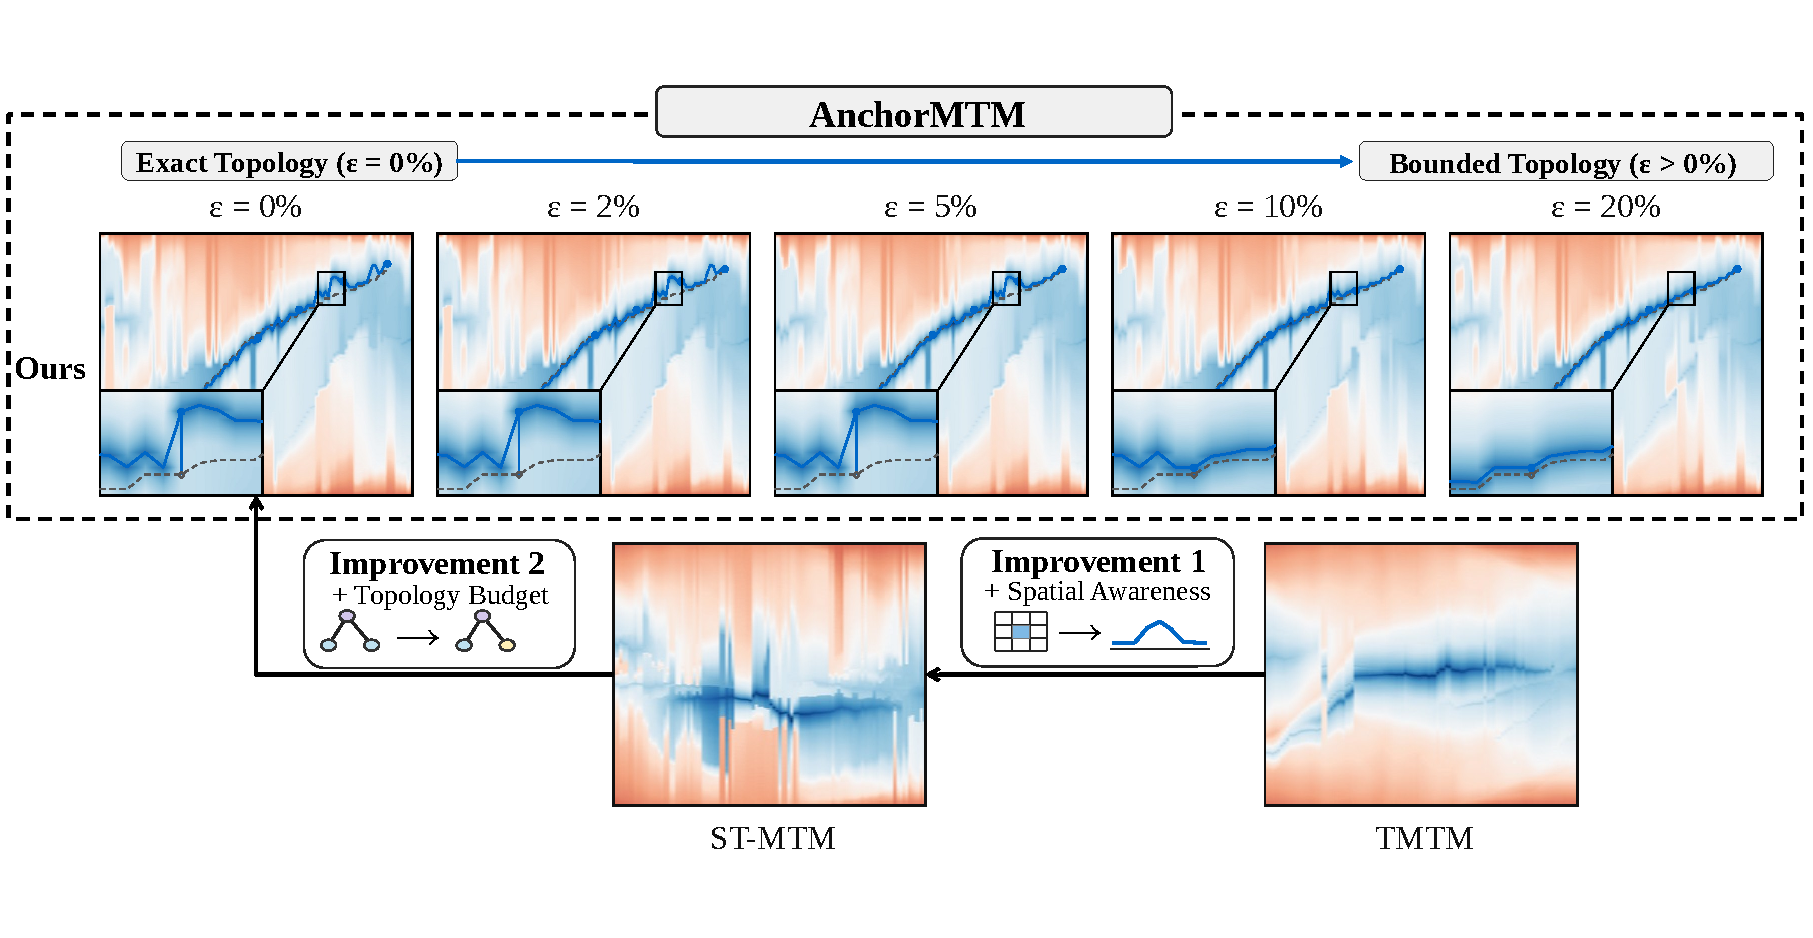
\includegraphics[width=\textwidth]{../figures/anchor_storms_budget_maps.pdf}
\caption{Storms 的参数地图与方法比较。AnchorMTM 覆盖精确拓扑（$\varepsilon=0$）和有界拓扑（2、5、10 和 20\%），配有原始轨迹和共同的局部放大。TMTM 和 ST-MTM 地图通过本地实现，使用相同的标量场和增广树。“空间感知”和“拓扑预算”表示各自概念上的改进。所有地图显示第 355--460 帧，使用原始蓝–橙色标，$[-35,35]$ hPa。模块之间的连接概括设计上的差异，并不表示严格的代数等价；多叉树适配器在正文中说明。}
\label{fig:storms-budget-profiles}
\end{figure}

\begin{figure}[t]
\centering
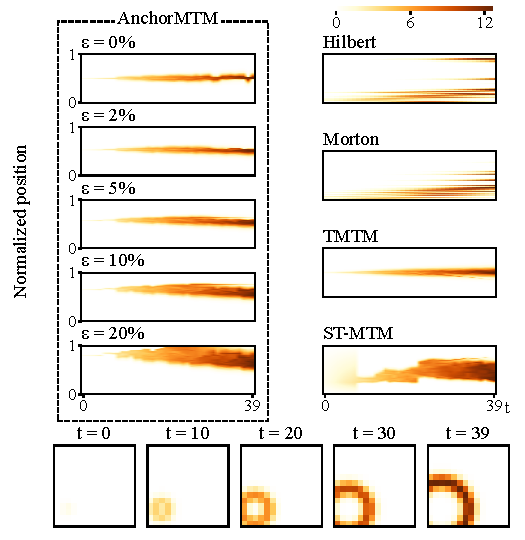
\includegraphics[width=0.6\textwidth]{../figures/anchor_ring_result.pdf}
\caption{Ring 比较。左：AnchorMTM 的拓扑允许量 $\varepsilon$ 与引导强度 $\alpha=\varepsilon/20\%$ 一起增大，从中性的中心目标（$\alpha=0$）到完整的空间引导（$\alpha=1$）；向上的移动反映的是引导，不只是允许量。右：提供的 Hilbert/Morton 参考面板，以及同输入的本地 TMTM/ST-MTM 结果。下：第 0、10、20、30 和 39 帧的源场快照。所有计算出的地图都使用 40 帧和 196 个位置；色标适用于计算出的地图和快照。纵坐标表示归一化的布局位置或曲线序号。}
\label{fig:ring-result}
\end{figure}

\paragraph{模式选择。}
对四个平面数据集，Exact 使用 $\varepsilon=0$。Balanced 在时间上前四分之一的帧上，从 1--10\%（步长 1\%）中选择一个正的预算。在实际 NMLE$_{\max}\le\varepsilon$ 的合法重建中，它最小化
\begin{equation}\label{eq:balanced-validation-score}
J=0.5\,\mathrm{NPE}_{norm}+0.5\,\mathrm{SNS}_{norm}.
\end{equation}
各项在合法候选上做最小–最大归一化；常数项贡献为零。在最小值 0.01 以内时，依次按较小的预算和实际误差打破并列。预算在完整运行之前冻结，没有退回零预算的选项。完整结果包含验证帧；此前的输出已被看到过，所以这不是新的盲测。

\subsection{参考定位与空间质量}
在全部四个输入上，ST-MTM 报告的 TW 都高于 AnchorMTM。它发表的 SNS 高于我们的本地值，但这些值来自作者的输入和帧覆盖，因此我们不跨来源对 SNS 或 TW 排名；Wildfires 上 Exact 的 TW 为 0.9136，也与发表的两位小数 0.91 太接近，不足以说明优势。

与固定方向的 Hilbert 和 Morton 曲线相比，Balanced 在 Gaussian、Wildfires 和 Storms 上的 SNS 和 TW 都更好。Ring 是例外：Hilbert 的 SNS 为 0.1252、TW 为 0.9048，而 Balanced 为 0.1334 和 0.8571；Ring 的 TW 只基于一个合格帧。在每个输入上，Balanced 的 NPE 都低于两条曲线和两个合并树适配器。相对 ST-MTM 适配器的降低分别为 92.3\%、84.0\%、96.3\% 和 96.9\%。这支持的是与指定参考的对齐，而不是一般意义上的可视化质量：遍历坐标不一定代表物理投影，相对几何也不能确定绝对原点。

\subsection{与 TMTM 的体数据比较}
%%TABLE_VOLUME%%
表~\ref{tab:volume-comparison} 沿用平面表的指标顺序和 Exact--Balanced 分组，但只与本地适配的 TMTM 比较。三个指标都在完整序列上重新计算；SNS 使用三维支撑质心距离，TW 取 $k=1$ 并覆盖全部帧，NPE 使用沿共同 $x$ 轴的极值目标。在两个数据集上，Balanced 的 SNS 和 NPE 都低于 TMTM，TW 都高于 TMTM。Exact 和 Balanced 使用相同的轴、树、保留的叶身份和布局权重，只有合并允许量不同。Exact 测得的固定叶合并误差为零，两个存储的 Balanced 结果都满足声明的拓扑预算。Tangaroa 较大的允许量（33.33\%）和以几何为主的目标限制了结论的归因：这些是选定的配置，既不说明普遍优越，也不是与平面默认权重的受控比较。

\subsection{拓扑有效性与放宽的效果}
Exact 的固定叶合并矩阵误差为零。Balanced 达到的最大 NMLE 为 0、0.982\%、4.421\% 和 9.985\%，都在各自的允许量之内；全部八次运行都通过了连续和栅格检查，没有重合的锚点。检查包括对角线上的极值，但不包括每一个增广的内部标签。Ring 在 26 个 Exact 帧和 21 个 Balanced 帧中需要经过检查的联合整数取整，保持其 196 个位置和连续的叶序。

Balanced 相对 Exact 的 NPE 降低：Ring 16.2\%，Wildfires 11.6\%，Storms 64.9\%。Gaussian 虽有 1\% 的正预算，结果不变。SNS 在 Ring 和 Storms 上改善，但在 Wildfires 上从 0.0426 升到 0.0447。因此放宽预算并不改善每一个指标。

这些 Exact--Balanced 比较衡量的是选定允许量的效果，而不是组件消融。正的允许量不一定改变选定的叶序，也不一定改善参考定位。预算约束的是合并层级误差，并不直接约束空间位移。

\subsection{位置界的准确性}\label{sec:bounds-eval}
\begin{figure}[t]
\centering
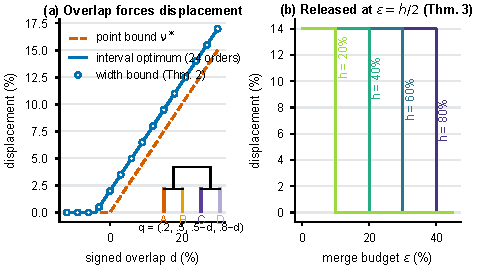
\includegraphics[width=0.55\textwidth]{../figures/anchor_controlled_bounds.pdf}
\caption{受控四叶树（插图：兄弟对和参考位置）。(a) 兄弟范围的重叠 $d$ 越大，迫使的位移越大；定理~\ref{thm:width} 的宽度界（圆圈）等于全部 24 种叶序中的最优值。(b) $d=24\%$ 时，14\% 的位移恰好在合并预算达到父间隙 $h$ 的一半时消失，四种间隙都如此，与定理~\ref{thm:chain} 的预测一致。百分比相对单位画布或单位标量范围。}
\label{fig:controlled}
\end{figure}
\emph{受控树。}为了分开位移的各个来源，我们固定两个兄弟对 $\{A,B\}$ 和 $\{C,D\}$，它们在根（层级 1）之下 0.4 处合并，叶值为 0，在单位画布上的参考为 $(0.2,0.5,0.5-d,0.8-d)$，并让带符号的重叠 $d$ 从 $-0.12$ 变到 $0.30$。在 43 个重叠值和四种宽度下，我们把下界与全部 24 种叶序比较，每种叶序都用一个独立的极小极大线性规划放置。仅拓扑就恰好迫使 $\nu^*=\max(0,d)/2$。宽度 0.06、间隔 0.01、$\rho=0.5$ 时，宽度界、我们的搜索和穷举最优重合于 $\tau=\max(0,(d+0.04)/2)$（图~\ref{fig:controlled}a）：$d=0.24$ 时点模型为 12\%，区间模型为 14\%。合并允许量恰好在定理~\ref{thm:chain} 允许交错的地方消除冲突，即对测试的四种父间隙 $h$ 都在 $2\varepsilon=h$ 处（图~\ref{fig:controlled}b）。

\emph{真实树。}我们还在一个早期基准的各帧上评估下界，所有序列使用同一个默认配置（补充材料）：五个平面序列共 614 帧，分别是 12 小时间隔的 ERA5 海平面气压~\cite{Hersbach:2020:ERA5}、逐日野火辐射功率~\cite{Franke:2021:1DP}、向外长波辐射~\cite{NOAA:OLR}、PM$_{2.5}$ 浓度~\cite{Dong:2026:PM25} 和 Ring，以及 Tangaroa 和 Cylinder 两个体数据。在精确模式下，614 个平面帧中有 606 帧所选叶序的区间代价 $\tau$ 等于 $\mathcal{B}_w$，因此在这些帧上没有任何精确拓扑叶序的最坏位移更小；$\varepsilon=10\%$ 时有 596 帧达到有界拓扑证书。体数据的树更难：Cylinder 的 102 帧中有 81 帧、Tangaroa 的 201 帧中有 27 帧达到下界，剩余的差距可能来自下界，也可能来自搜索。由于定理~\ref{thm:order} 不需要布局，它也能衡量已有的地图：中点排序在同一棵树上达到 $\nu^*$，所以高于 $\nu^*$ 的顺序误差是由排序规则选择的，而不是层次迫使的。在这七个序列上，TMTM 的顺序误差有 53--95\%、ST-MTM 有 31--95\% 高于 $\nu^*$，每张图都按与参考更一致的镜像方向计算。

\subsection{Ring 案例：时序概览与源场快照}
图~\ref{fig:ring-result} 展示 Ring 上引导与拓扑的联合扫描：$\varepsilon=0,2,5,10,20\%$，引导强度 $\alpha=\varepsilon/20\%$。布局目标在画布中点与固定的 $-128.7^\circ$ 物理投影之间插值：$q_{layout}=(1-\alpha)q_{mid}+\alpha q_{physical}$。因此更强的引导通过实际优化（而不是平移图像）把重建出的环向上移。这一定性扫描同时改变引导和拓扑允许量，每个面板都标出了两个值；它不是只改变 $\varepsilon$ 的消融，其中 $\alpha=0$ 的面板也不是表~\ref{tab:quantitative-final} 中的精确模式，它也不替代主表冻结的设置。TMTM/ST-MTM 地图使用相同的场和树；Hilbert/Morton 仍是提供的参考图。五张源场快照显示了环的扩张和增强。

\subsection{Storms 案例：解读带预算的地图}
图~\ref{fig:storms-budget-profiles} 上排保留了图~\ref{fig:storms_overview} 中原有的五档预算 Storms 定性档案，与主表的预处理不同。0、2 和 5\% 的布局在局部重合，而 10 和 20\% 把选定的特征移向它的固定参考。下排是在同样 744 个标量场和增广树上重新计算的 TMTM 和 ST-MTM 地图，显示相同的事件时段，没有逐面板重新着色或平移。TMTM 用基于重叠的时间子树对齐代替锚定放置；ST-MTM 使用基于几何的排序和考虑距离的放置，并带时间位置约束。本地 TMTM 实现用同层级的分隔副本处理真正的多叉鞍点；ST-MTM 适配器把它们细化为编号稳定的同层级二叉层次，并核对原始叶的最低公共祖先矩阵。两个基线都从第 40 帧开始，显示栅格为 8192 个位置。它们是本地实现，不是作者的程序。模块箭头描述的是替换和增加，不声称严格的算法归约，也不改变主表的协议。

\subsection{参数与计算代价}
表~\ref{tab:anchor-parameters-final} 列出四个平面数据集的 Balanced 预算（1、1、5 和 10\%）和布局参数；表~\ref{tab:volume-parameters} 单独列出体数据集及其设置。平面表报告在 Apple M4 上一次无缓存的 Balanced 运行，使用一个 BLAS/TTK 线程、顺序提取和默认的 HiGHS 调度器。优化时间包括排序和放置；总时间还包括预处理、建树、匹配/参考估计、栅格化、读写和检查。不含导入、报告和指标导出；操作系统缓存可能是热的。这些计时不能说明加速的显著性。基线的 NPE 使用公开说明的 CompactTMTM 和 ST-MTM 求解器适配，不是作者的程序。

\section{讨论与局限}
下界把迫使的位移与选择的位移分开。高于 $\nu^*$ 的顺序误差总能在不改变树的情况下消除，因为中点排序达到 $\nu^*$；宽度感知界和有界拓扑界不一定能达到，所以高于它们的部分可能在于下界本身，而不在于布局。由于它们不需要布局，可以在画任何地图之前，对候选参考方向计算。

固定的物理参考和以几何为导向的嵌入回答不同的问题。AnchorMTM 支持沿选定空间坐标读取位置；ST-MTM 报告的较高 TW 说明了保持局部邻域的价值。两种性质互不保证。因此四个输入上的结果支持的是针对特定任务的锚定主张，而不是在空间或时间保真度上普遍更优。

实证比较有三个局限。第一，作者处理后的场及其小样本 TW 协议无法完整获得，所以发表的 SNS/TW 不能提供同一输入下的显著性检验。第二，参考和追踪由给定序列离线计算；支撑重叠是对应关系的代理，而不是物理身份的标注。第三，叶序搜索是启发式的，连续证书不能消除整数渲染的约束。我们在重建后检查实际的固定标签合并矩阵，但不对每一个增广内部标签给出证书。

实验也没有证明感知上的可读性、对物理运动判断的准确性、重复运行的加速，或对未见数据集的泛化。这些需要单独的研究。扩展这一评估时，有必要把源数据来源、覆盖范围、失败的候选和实际的拓扑误差与数值分数一起保存。

\section{结论}
AnchorMTM 给时序合并树图一条空间轴，并说明它的代价：三个下界给出精确拓扑、有限宽度和有界合并误差在任何布局上迫使的位移。在 614 个真实平面帧中，有 606 帧所选的精确拓扑叶序达到宽度感知下界；TMTM 和 ST-MTM 的顺序误差有 31--95\% 不是树迫使的。在四个本地输入上，这些布局在每个声明的合并预算之内，相比同输入的基线适配器改善了绝对参考定位；而 ST-MTM 已发表的邻域保持指标仍然更高。

\bibliographystyle{abbrv-doi-narrow}
\bibliography{../refs}
\end{document}
